\documentclass{ieeeaccess}
\usepackage{cite}
\usepackage{amsmath,amssymb,amsfonts}
\usepackage{graphicx}
\usepackage{textcomp}
\usepackage{array}
\usepackage{multirow}
\usepackage{booktabs}
\usepackage{float}
\usepackage{placeins}
\usepackage{url}
\usepackage{etoolbox}
\usepackage{hyperref}
\hypersetup{colorlinks=true,citecolor=blue,linkcolor=blue,urlcolor=blue}
\graphicspath{{figures/}{./}}
\tolerance=9999
\emergencystretch=4em
\hbadness=10000
\vbadness=10000
\hfuzz=12pt
\vfuzz=12pt

\renewcommand{\topfraction}{0.9}
\renewcommand{\bottomfraction}{0.8}
\renewcommand{\textfraction}{0.1}
\renewcommand{\floatpagefraction}{0.9}
\setcounter{topnumber}{3}
\setcounter{bottomnumber}{2}
\setcounter{totalnumber}{5}

\usepackage{bm}
\makeatletter
\AtBeginDocument{\DeclareMathVersion{bold}
\SetSymbolFont{operators}{bold}{T1}{times}{b}{n}
\SetSymbolFont{NewLetters}{bold}{T1}{times}{b}{it}
\SetMathAlphabet{\mathrm}{bold}{T1}{times}{b}{n}
\SetMathAlphabet{\mathit}{bold}{T1}{times}{b}{it}
\SetMathAlphabet{\mathbf}{bold}{T1}{times}{b}{n}
\SetMathAlphabet{\mathtt}{bold}{OT1}{pcr}{b}{n}
\SetSymbolFont{symbols}{bold}{OMS}{cmsy}{b}{n}
\renewcommand\boldmath{\@nomath\boldmath\mathversion{bold}}}
\makeatother

\def\BibTeX{{\rm B\kern-.05em{\sc i\kern-.025em b}\kern-.08em
    T\kern-.1667em\lower.7ex\hbox{E}\kern-.125emX}}

% Suppress the template's "VOLUME X, YYYY" footer line; IEEE sets it at production.
\makeatletter
\AtBeginDocument{%
  \def\@oddfoot{\raisebox{8pt}{%
    \hbox to 0pc{\hbox to \textwidth{\mbox{}\hfill{\footerpagefont\thepage}}}}}%
  \def\@evenfoot{\raisebox{8pt}{%
    \hbox to 0pc{\hbox to \textwidth{{\footerpagefont\thepage}\mbox{}\hfill}}\hspace*{1.8pc}}}%
}
\makeatother

%Your document starts from here ___________________________________________________
\begin{document}
% Publication history and DOI are assigned by IEEE Access at production time;
% the lines below hold neutral placeholders required by the template macros.
\history{}
\doi{}

\title{A Privacy-First Edge-AI Home Security System on Raspberry Pi~5 with Hailo-8L NPU}
\author{\uppercase{Gonugondla Veera Manikanta}\authorrefmark{1}, \uppercase{Swathi Tangi}\authorrefmark{1}}

\address[1]{Manipal Institute of Technology, Manipal Academy of Higher Education, Manipal, India}

\markboth
{G.V. Manikanta \emph{et al.}: A Privacy-First Edge-AI Home Security System on Raspberry Pi~5 with Hailo-8L NPU}
{G.V. Manikanta \emph{et al.}: A Privacy-First Edge-AI Home Security System on Raspberry Pi~5 with Hailo-8L NPU}

\corresp{Corresponding author: Swathi Tangi (e-mail: swathi.tangi@manipal.edu).}


\begin{abstract}
Consumer home security is split between cloud-subscription cameras that stream every frame off-site and do-it-yourself single-board builds that rarely advance past frame-differencing motion detection; the former forfeits privacy, the latter forfeits recognition accuracy, secondary verification, and hardened remote access. This paper addresses that gap with a privacy-first edge-AI reference platform on which every frame of inference stays on the device and no image or video data ever leaves it. The platform runs on a Raspberry~Pi~5 paired with a Hailo-8L neural processing unit (13~TOPS, INT8), and integrates YOLOv8s as the primary four-class detector, MobileNetV2 as a secondary weapon-crop verifier, and MiDaS~Small as a depth-variance pre-filter, dispatched through GStreamer and the Hailo TAPPAS framework; the services layer is a FastAPI stack behind a Cloudflare tunnel, with PBKDF2-SHA256 plus one-time-password authentication and AES-256-GCM encrypted evidence clips. Real-time behaviour is obtained by pairing an asynchronous, CPU-pinned, bounded-queue pipeline with an INT8 compilation of the detector to a 22.9~MB Hailo executable format binary that isolates the accelerator path from the host services. On the held-out four-class test split, the on-chip run reports mAP{@}0.5 = 0.854 and mAP{@}0.5:0.95 = 0.682, within $+0.007$ and $+0.012$ of the FP32 reference, and sustains 52.2~FPS at 18.4~ms on-chip latency. Under concurrent SMTP, SSH, voice, and streaming load it holds $52.26 \pm 0.76$~FPS across six operating modes with zero camera-side frame drops. The contribution is a measured, reproducible systems-integration result on commodity edge hardware rather than a new detector or algorithm.
\end{abstract}

\begin{keywords}
Edge AI, Hailo-8L, Raspberry Pi, Object detection, Privacy-preserving computing.
\end{keywords}

\titlepgskip=-21pt

\maketitle

\section{Introduction}
\label{sec:introduction}
\PARstart{H}{ome} security has moved a long way from the passive siren-plus-passive-infrared boxes of the 1990s, yet the consumer market remains sharply partitioned. Cloud-backed products from large vendors stream every frame of footage to a remote data centre and bill the user a monthly subscription, leaving the owner with almost no control over the raw video. Do-it-yourself builds on single-board computers keep the data local and the cost low, but most never advance past frame-differencing motion detection and therefore lack second-stage reasoning, a voice interface, or an encrypted evidence path. Dedicated neural processing units are now closing that gap, bringing deep-learning inference to the edge at single-digit watts and at a price a hobbyist can absorb, so that real-time multi-class detection, a secondary verifier, and a full services stack can share one privacy-preserving single-board platform.

The prior art that this paper builds on falls into five strands: edge-deployed YOLO detectors, the dispatch framework and host hardware, visible-weapon detection in surveillance, face anti-spoofing and the verifier building blocks, and adjacent systems-level smart-home work.

Since the original YOLO formulation~\cite{b2}, the detector family has been ported to a range of edge accelerators. FL-YOLO on a Jetson TX1 reaches 36.7~FPS at 76.7\% AP in a coal-mine edge-cloud framework~\cite{b1}; YOLOv3-Tiny on a Xilinx Kria KV260 FPGA sustains 15~FPS at 99\% accuracy at 3.5~W~\cite{b5}; and PG-YOLO compresses YOLOv5s by $9\times$ at only 0.1\% accuracy loss through Ghost modules, pruning, and distillation~\cite{b6}. Cross-accelerator benchmarks~\cite{b25,b26} further confirm that Jetson Orin Nano delivers higher raw FPS at 3--4$\times$ the idle power of a Pi plus accelerator, and that Coral TPU is constrained by its INT8-only op surface on YOLOv8-class heads. Transformer-augmented surveillance models~\cite{b27} and pruned-quantised Pi deployments~\cite{b29} show that edge-compatible post-processing remains achievable within tight compute envelopes.

The baseline detector used here is the Ultralytics YOLOv8 framework~\cite{b9}, dispatched through the Hailo TAPPAS (Template Applications, APIs, Pipelines, and Solutions) framework~\cite{b10} on top of GStreamer~\cite{b13}. The host platform is a Raspberry~Pi~5~\cite{b11} paired with a Hailo-8L accelerator, which Bueno \emph{et~al.}~\cite{b4} report, on a low-cost microscopy benchmark, to be accuracy-competitive with GPU systems at a fraction of the power draw; that study is a cross-domain precedent rather than a direct surveillance evaluation.

For visible-weapon detection, YOLOv4 on a curated CCTV corpus reaches F1 = 0.91~\cite{b18}; YOLOv5 with augmentation stabilises rare-class mAP~\cite{b30}; YOLOv7-DarkVision reaches 95.5\% precision under low light~\cite{b19}; YOLOv4 with hand--weapon heuristics plus classical classifiers cuts armed-person false positives~\cite{b20}; and the ACF benchmark supplies a surveillance-perspective corpus~\cite{b32}. The closest hardware precedent deploys a customised YOLOv8 gun/knife detector on a Raspberry~Pi~4 without NPU offload, verifier, or anti-spoof stage~\cite{b28}.

Face anti-spoofing surveys~\cite{b21} report intra-dataset ACER in the 1--2\% range with cross-dataset generalisation still open; the CelebA-Spoof benchmark~\cite{b22} and recent test-time domain generalisation work~\cite{b23} frame that gap. This paper does not claim a new anti-spoof method and uses MiDaS Small~\cite{b14} only as a depth-variance pre-filter, with MobileNetV2~\cite{b15} as the secondary verifier.

At the systems level, occupant-aware smart-home deployments~\cite{b31} and the Frigate NVR~\cite{b24} show adjacent work. The former depends on a cloud classifier; the latter runs local detectors on Coral TPU or TensorRT back-ends, but as an integration platform it does not publish an INT8 latency budget under concurrent service load. The capability gap addressed by this paper combines the five strands above: an INT8-deployed four-class detector, a secondary weapon-crop verifier, and a depth-plus-colour pre-filter, co-resident on one sub-10~W NPU-equipped single-board computer alongside FastAPI~\cite{b12}, Cloudflare-tunnel remote access~\cite{b17}, authenticated voice, and encrypted-evidence services, with per-stage latency and FPS-flatness measured under that concurrent load.

The contribution of this paper is deliberately scoped as a \emph{measured systems-integration result on commodity edge hardware}, not a new detector, compression technique, or anti-spoof algorithm. YOLOv8s, MobileNetV2, MiDaS~Small, GStreamer/TAPPAS, FastAPI, Cloudflare-tunnel ingress, PBKDF2-SHA256, and AES-256-GCM are all used as published; the novelty is in how they are co-resident, measured, and bounded on one sub-10~W single-board platform. Concretely, this paper contributes:
\begin{itemize}
\item \emph{An integration architecture.} An asynchronous, CPU-pinned, bounded-queue design that co-locates a primary detector, a secondary verifier, and a depth-variance pre-filter on one 13~tera-operations-per-second (TOPS) Hailo-8L device while a FastAPI web stack, a voice assistant, authentication, remote-access, encrypted-evidence, and logging services run on the same Raspberry~Pi~5, with the NPU path and the CPU services engineered to be non-interfering by construction.
\item \emph{An INT8 deployment characterisation.} A four-class domestic-threat YOLOv8s detector compiled to a 22.9~MB Hailo executable format (HEF) binary, re-evaluated on-chip on the held-out test split, with measured mAP{@}0.5 = 0.854 and mAP{@}0.5:0.95 = 0.682, within $+0.007$ and $+0.012$ of the FP32 reference values 0.847 and 0.670 (Section~\ref{sec:quant}).
\item \emph{A per-stage latency and throughput budget} for the on-chip cascade: 52.2~FPS at 18.4~ms primary detection, with the MobileNetV2 verifier and MiDaS pre-filter sharing the same device inside a detect-to-decision envelope of 22--27~ms.
\item \emph{An FPS-flatness result under concurrent service load}: $52.26 \pm 0.76$~FPS across six operating windows (Baseline, Idle, DND, Privacy, Emergency, Active) with zero camera-side frame drops, measured while SMTP alerts, AES-encrypted SFTP clip uploads, voice queries, and an MJPEG pull run concurrently on the CPU side.
\end{itemize}
The boundary of what is \emph{not} claimed is stated explicitly in Section~\ref{sec:results}: no new algorithm, no continuous-deployment alert precision/recall, no nuisance-condition sweep, and no face anti-spoof decision (the MiDaS stage is used only as a cheap depth-variance pre-filter and is bounded in Section~\ref{sec:antispoof_eval}).


\section{Methodology}
\label{sec:methodology}
This section gives two high-level views of the system before the detailed engine-by-engine methodology. Fig.~\ref{fig:block_diagram} shows the three-layer block diagram, organising the system by architectural role. Fig.~\ref{fig:system_flowchart} traces the runtime path of a detection event.

The three-layer split is not a product diagram. It is the partition that makes the empirical claims of this paper testable in isolation. The top (inference) layer is the only consumer of NPU time, so the per-stage latency budget in Section~\ref{sec:results} can be attributed to a single resource path. The middle (response and control) layer contains the event-driven components whose mode-gating semantics decide whether a given detection produces downstream work, and therefore carries the overhead attributable to idle and DND modes. The bottom (web server and persistence) layer carries all outward-facing traffic: FastAPI~\cite{b12}, the Cloudflare tunnel~\cite{b17}, authentication, the deadman watchdog, and the logging engine. It is also the source of the concurrent CPU load against which the FPS-flatness result of Section~\ref{sec:async_fps} is measured.

\begin{figure}[htbp]
\centering
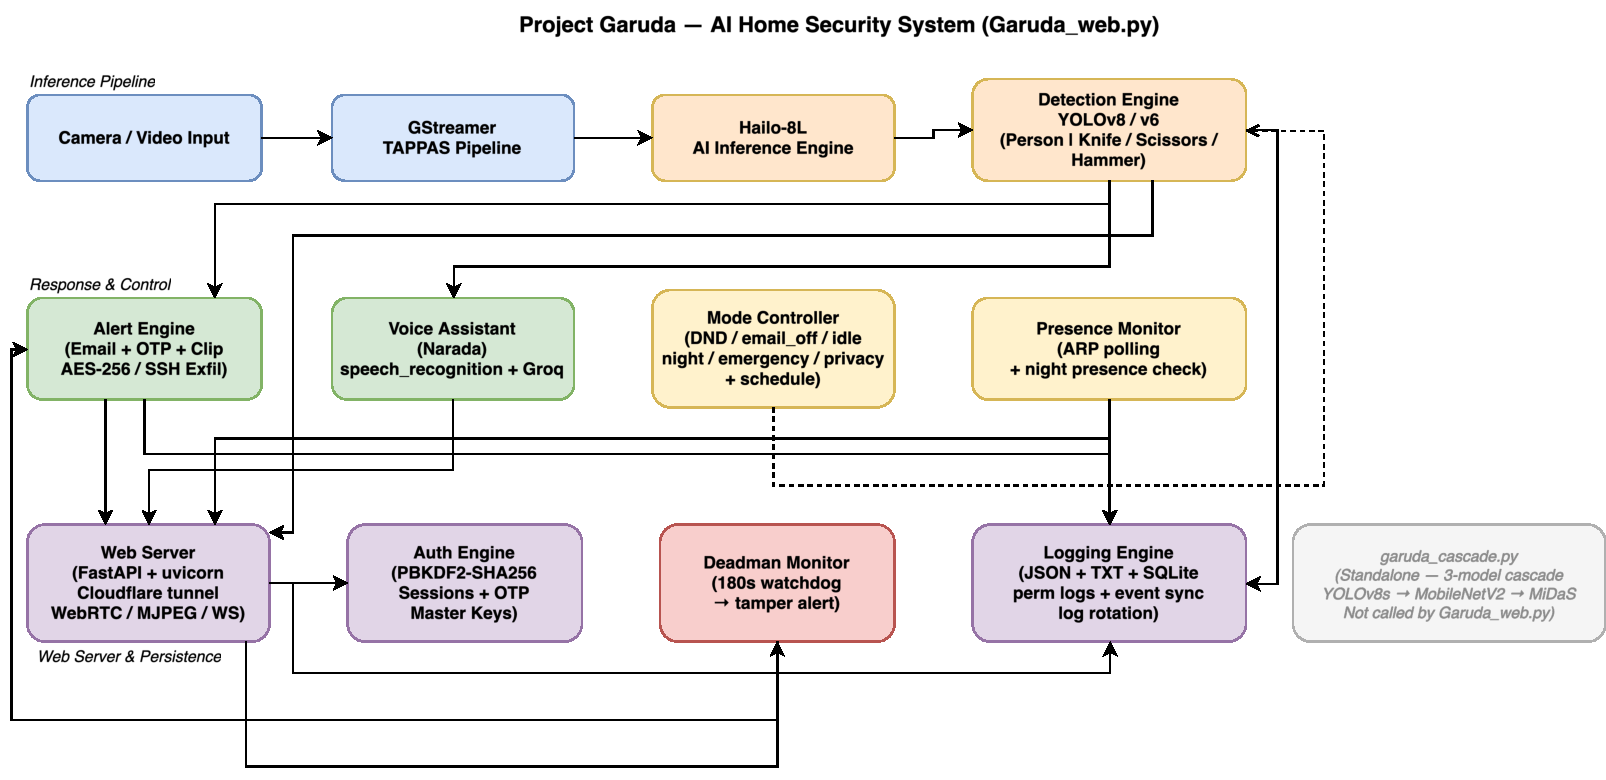
\includegraphics[width=\columnwidth,keepaspectratio]{garuda_block_diagram.drawio-3.pdf}
\caption{Three-layer block diagram of the proposed system.}
\label{fig:block_diagram}
\end{figure}

Fig.~\ref{fig:system_flowchart} traces the runtime path of a single detection event so that the latency numbers in Section~\ref{sec:results} can be located on the diagram. Frames enter the GStreamer TAPPAS pipeline from the Raspberry Pi Camera Module~v3 and are classified on the Hailo-8L by YOLOv8s with non-maximum suppression (NMS) at $\text{IoU} \le 0.45$ and confidence $\ge 0.25$. Outputs are partitioned into watch labels (Person) and danger labels (Knife, Scissors, Hammer); a danger detection that passes both the three-consecutive-frame gate and the active mode check enters the alert fan-out path. The remaining CPU-side services (Section~\ref{sec:cpu_services}) run off the inference thread and are the load against which the FPS-flatness result of Section~\ref{sec:async_fps} is measured.

\begin{figure}[htbp]
\centering
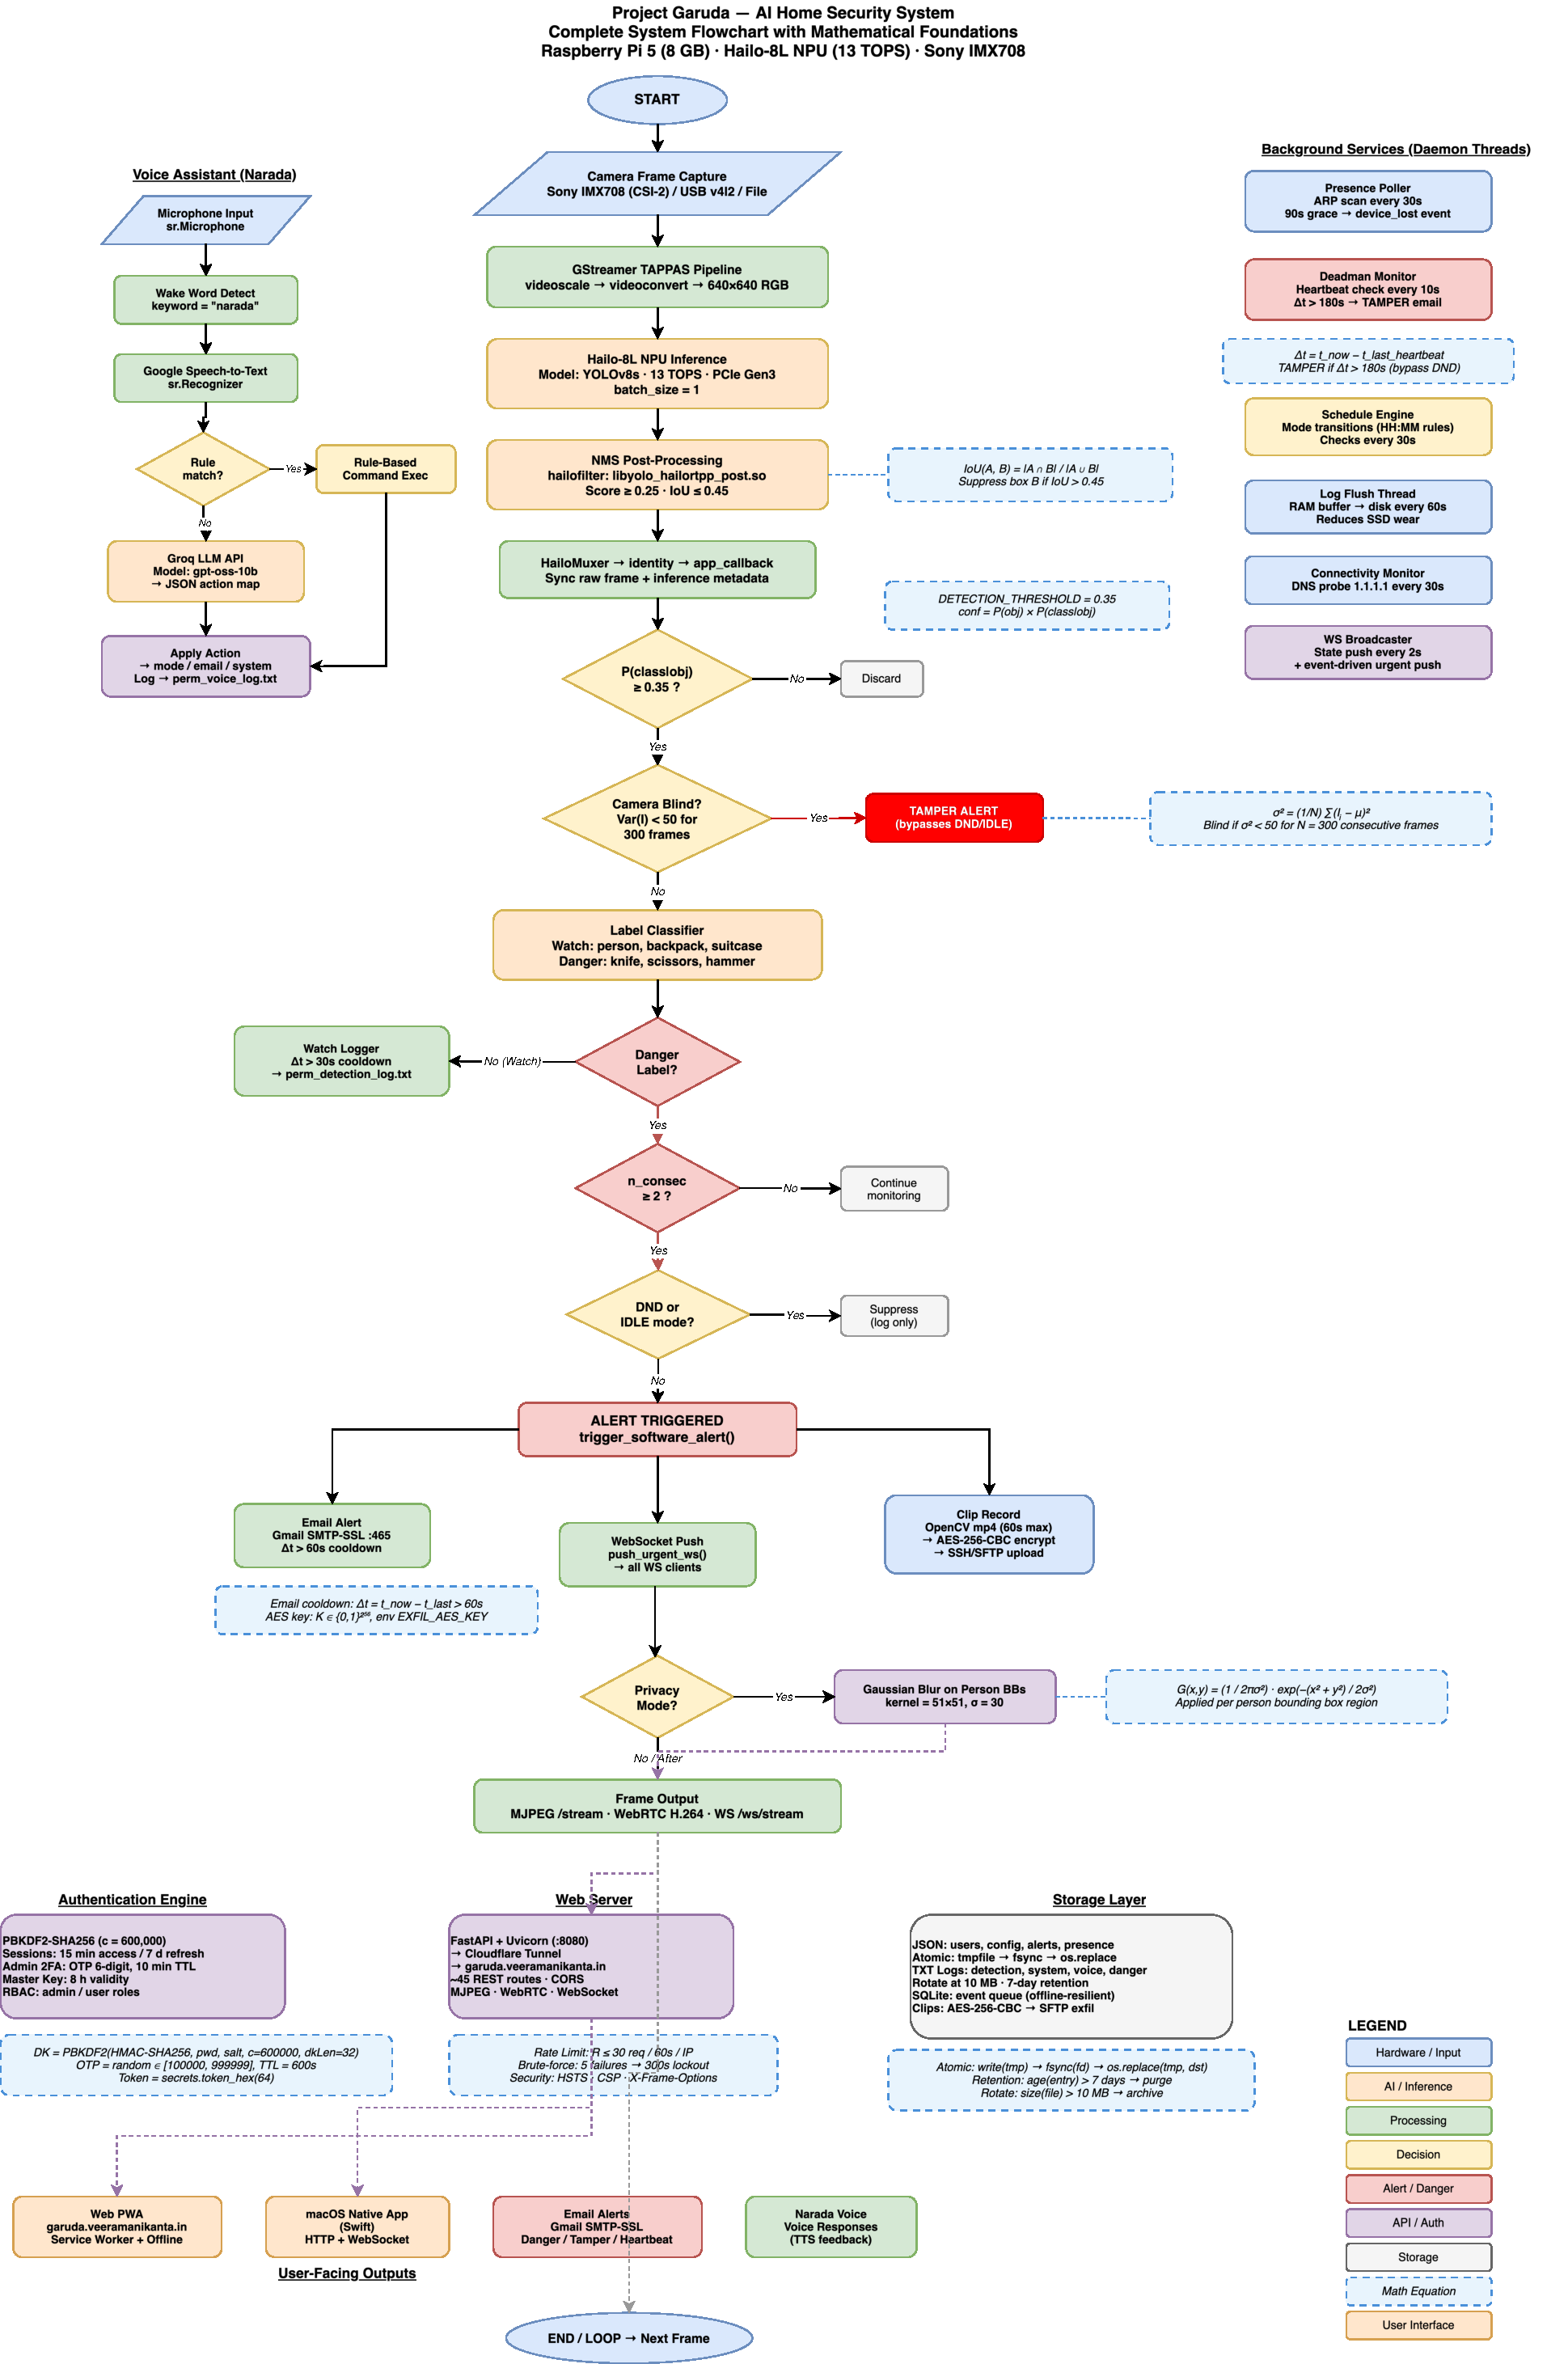
\includegraphics[width=\columnwidth,height=\textheight,keepaspectratio]{garuda_system_flowchart.drawio.pdf}
\caption{End-to-end runtime diagram of a danger event.}
\label{fig:system_flowchart}
\end{figure}

\subsection{Dataset}
\label{sec:dataset}
The detector is trained on a four-class corpus (Hammer, Knife, Person, Scissors), referred to as v5, covering the objects a home-surveillance user is most likely to want flagged. The corpus was assembled in three reported passes (v1, v2, v5); intermediate builds v3 and v4 were discarded as ablation snapshots and are not evaluated here. The resulting dataset-size progression is revisited as an experimental variable in Section~\ref{sec:results}.

\subsubsection{Source Datasets}
\label{sec:sources}
Training imagery was drawn from two public, permissively licensed sources, merged into a single four-class schema before training. Each import was reviewed, filtered, and re-annotated where necessary.

\textbf{Source A --- Roboflow ``Knives \& Scissors Training v2.''} CC BY 4.0 Roboflow Universe dataset with classes Hammer~(0), Knife~(1), Person~(2), and Scissors~(3), shipped in YOLO-v5 normalised label format with an upstream 359 / 102 / 51 split. Predominantly 640$\times$640 studio-lit JPEGs; the seed established the annotation convention but was class-imbalanced and visually narrow. The upstream split labels are discarded during ingestion: all Roboflow images (including dataset-side augmentation variants) are pooled with Source~B and redistributed by the stratified 80/10/10 re-split of Section~\ref{sec:preprocess}, under which the Roboflow contribution registers as the 2{,}730-image entry of Table~\ref{tab:sources}.

\textbf{Source B --- OpenImages v7 (OIDv4 toolkit and FiftyOne).} Google-verified human annotations at IoB $\geq 0.5$, CC BY 4.0, exported in YOLO Darknet format per class. Contributes the real-world diversity missing from the Roboflow seed: 1{,}219 images in the v2 pass and a further 2{,}276 in the v5 pass, targeted at whichever class had the lowest mAP after the previous training run.

\begin{table}[ht!]
\caption{\textbf{Image Counts Contributed by Each Source (v5 Splits)}}
\label{tab:sources}
\setlength{\tabcolsep}{3pt}
\centering\small
\begin{tabular}{|l|c|c|c|c|}
\hline
\textbf{Source} & \textbf{Train} & \textbf{Val} & \textbf{Test} & \textbf{Total} \\
\hline
Roboflow seed (all four classes)     & 2{,}187 & 285 & 258 & 2{,}730 \\
OpenImages v7 --- Hammer             & 93      & 12  & 14  & 119   \\
OpenImages v7 --- Knife              & 495     & 49  & 56  & 600   \\
OpenImages v7 --- Person             & 1{,}981 & 245 & 259 & 2{,}485 \\
OpenImages v7 --- Scissors           & 226     & 31  & 35  & 292   \\
\hline
\textbf{All sources}                 & \textbf{4{,}982} & \textbf{622} & \textbf{622} & \textbf{6{,}226} \\
\hline
\end{tabular}
\end{table}

OpenImages class tags are noisy for close-up tool photographs, so automated import was unsafe. Every image was visually inspected before inclusion.

\paragraph*{Methodological Limits of the Dataset Study}
\label{sec:dataset_limits}
The v2$\rightarrow$v5 OpenImages additions were not drawn uniformly: after each run, imagery was pulled for whichever class had the lowest mAP. That reflects deployment-driven engineering rather than a randomised scaling sweep, and the per-class trajectory is shaped partly by the selection policy. The 80/10/10 stratified re-split uses a fixed seed (42) and a single draw, so the v1/v2/v5 test-mAP values are point estimates without confidence intervals; reported run-to-run variance for YOLO fine-tuning on similar corpora is $\pm 0.01$--$0.02$ mAP{@}0.5. The 0.382-point jump from v1 to v5 exceeds the upper envelope bound of $\pm 0.02$ by a factor of $0.382 / 0.02 \approx 19$, but the intermediate v2 waypoint and the per-class ordering are not statistically resolved. Inclusion was author-curated, so the result measures generalisation within one curation policy and one corpus. A repeated-seed, repeated-split re-analysis, an inter-annotator-agreement check, and an external-benchmark evaluation are flagged as future work in Section~\ref{sec:conclusion}.

\subsubsection{Preprocessing and Validation Pipeline}
\label{sec:preprocess}
Preprocessing must reconcile three constraints: the Hailo-8L accepts a fixed 640$\times$640 INT8 input, the IMX708 camera delivers 16:9 frames, and YOLO labels must stay geometrically correct after resize. A naive $640\times640$ resize on a $4608\times2592$ OpenImages photo compresses the horizontal axis by $7.2\times$ and the vertical axis by $4.0\times$, destroying bounding-box aspect ratios. Letterboxing preserves aspect by padding the shorter axis with grey pixels, in five steps.

\textit{Step 1 --- Letterbox resize.} Each image is scaled by $s=\min(640/W,\,640/H)$, placed in a 640$\times$640 canvas, and padded with the YOLO-standard grey fill $(114,114,114)$ so training- and inference-time padding match.

\textit{Step 2 --- Label coordinate remap.} YOLO-normalised coordinates are remapped to the padded canvas as $c_x^\prime = (c_x \cdot s + p_x)/640$ and equivalently for $c_y, b_w, b_h$, then clamped to $[0.001, 0.999]$ to avoid a boundary-value condition inside YOLOv8's loss.

\textit{Step 3 --- Integrity and deduplication.} Images are decode-checked with OpenCV, labels are parsed for YOLO validity, and a SHA-256 hash per image catches cross-split duplicates. One image was dropped from the v2 merge for a missing annotation; all other integrity checks passed.

\textit{Step 4 --- Stratified re-split (seed=42).} All sources are pooled and re-split at 80/10/10 with class-primary stratification. The fixed seed is reused across every dataset-version comparison.

\textit{Step 5 --- Filename namespacing.} Files are prefixed by source (\texttt{roboflow\_*}, \texttt{openimages\_knife\_*}, etc.) to keep the merge idempotent.

Training runs for 150 epochs (v5) or 200 epochs (v6), with the reported weights taken from the best-validation-mAP checkpoint rather than the final epoch; the plateau visible in Fig.~\ref{fig:training_metrics} confirms that pushing past that checkpoint does not recover additional test mAP.

Online augmentation uses YOLOv8 defaults: Mosaic at probability~1.0, horizontal flip at 0.5, HSV jitter ($h{=}0.015$, $s{=}0.7$, $v{=}0.4$), scale~0.5, and translate~0.1. MixUp is disabled after early experiments showed label noise when combined with Mosaic. No rotation or shear is applied.

\subsubsection{Final Dataset Geometry}
\label{sec:dataset_geometry}
The final v5 dataset contains 6{,}226 JPEG images (4{,}982 train, 622 val, 622 test) with 5{,}311 annotated instances, totalling 1.32~GB. Native resolutions span 436--4{,}608~px wide and 303--3{,}456~px tall across 439 unique sizes; the most common is 640$\times$640 (43.9\%). All images are letterbox-resized to $640\times640$ before training.

Per-split, per-class instance counts are given in Table~\ref{tab:instances}. Person dominates with 2{,}100 training instances; Hammer is the rarest at 480, reflecting the relative frequency in public imagery. The distribution is visualised in Fig.~\ref{fig:dataset_dist}.

\begin{table}[ht!]
\caption{\textbf{Annotated Instance Counts per Class per Split}}
\label{tab:instances}
\setlength{\tabcolsep}{3pt}
\centering\small
\begin{tabular}{|l|c|c|c|c|}
\hline
\textbf{Class}  & \textbf{Train} & \textbf{Val} & \textbf{Test} & \textbf{Total} \\
\hline
Hammer   & 480     & 68      & 30    & 578    \\
Knife    & 860     & 122     & 60    & 1{,}042 \\
Person   & 2{,}100 & 302     & 173   & 2{,}575 \\
Scissors & 900     & 128     & 88    & 1{,}116 \\
\hline
\textbf{Total} & \textbf{4{,}340} & \textbf{620} & \textbf{351} & \textbf{5{,}311} \\
\hline
\end{tabular}
\end{table}

Table~\ref{tab:sources} and Table~\ref{tab:instances} report complementary quantities rather than the same figure twice: the former counts image files contributed by each source, while the latter counts annotated bounding-box instances per class. The lower instance-to-image ratio in the test split (351 instances over 622 images) reflects the natural variation in object density across the curated splits and does not indicate a missing-annotation issue.

\begin{figure}[ht!]
\centering
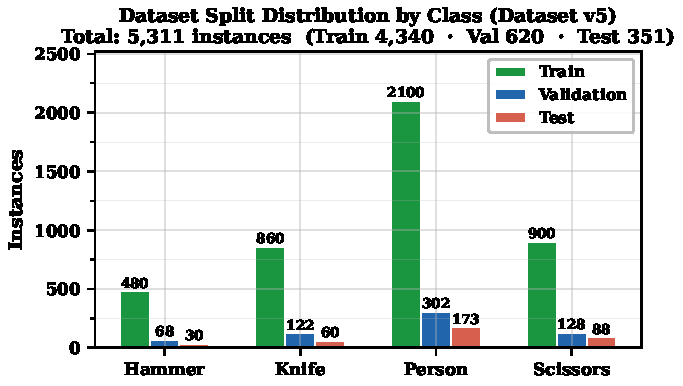
\includegraphics[width=\columnwidth]{fig8_dataset_distribution.pdf}
\caption{v5 dataset class distribution across splits (graphical view of the counts in Table~\ref{tab:instances}).}
\label{fig:dataset_dist}
\end{figure}

Person has the highest small-object fraction in the training split (5.2\% by COCO (Common Objects in Context)-style area thresholds, versus under 2.5\% for the other classes), driven by partial annotations and crowded scenes. Recall on this class is correspondingly hardest to recover (Section~\ref{sec:results}).

The MobileNetV2 Safe/Weapon classifier is trained on tight bounding-box crops from the YOLO training split. Weapon crops come from Hammer (150), Knife (731), and Scissors (667) detections; Safe crops are Person bounding boxes capped at 2{,}000. All crops are resized to $224\times224$. Training uses a single linear head (1{,}280$\to$2) on an ImageNet-pretrained backbone, in two phases: 5 head-only epochs (AdamW, lr$=$1e-3) and 35 full fine-tune epochs (AdamW, lr$=$3e-4, cosine annealing). Class imbalance is handled with focal loss ($\gamma{=}2.0$, $\alpha{=}[1.0,1.5]$) and a \texttt{WeightedRandomSampler}. Evaluation uses a 500-crop held-out set (250 Safe + 250 Weapon) drawn exclusively from the YOLO val/test splits, with zero overlap. The closed-set, crop-only distribution (no household negatives, no occlusions that would not reach this stage in deployment, no temporal video) bounds the headline classifier accuracy reported in Section~\ref{sec:classifier_eval}. The split is summarised in Table~\ref{tab:mobilenet}.

\begin{table}[ht!]
\caption{\textbf{MobileNetV2 Classifier Dataset (v2)}}
\label{tab:mobilenet}
\setlength{\tabcolsep}{4pt}
\centering\small
\begin{tabular}{|l|c|c|c|}
\hline
\textbf{Split} & \textbf{Safe crops} & \textbf{Weapon crops} & \textbf{Total} \\
\hline
Train    & 2{,}000 & 1{,}548 & 3{,}548 \\
Held-out & 250     & 250     & 500 \\
\hline
\end{tabular}
\end{table}


Engines are described in the order that video and control flow through the system. The inference path (hardware, GStreamer pipeline, detection callback, secondary verifier) is treated in detail; the remaining CPU-side services (alert, voice, mode control, presence, web server, authentication, deadman, logging) are sketched more briefly, because their contribution is in the integration rather than in any single algorithm. Design trade-offs are collected in Section~\ref{sec:design_decisions}.

\subsection{Hardware Engine}
The governing constraint is that neural inference must live on a dedicated accelerator so the quad-core CPU remains free for the web server, voice pipeline, and logging. A Raspberry~Pi~5 (Broadcom BCM2712, Cortex-A76) hosts the system under 64-bit Raspberry Pi OS, running at a sustained 2.8~GHz (\texttt{arm\_freq=2800}) with the official 5~V/5~A PSU and active cooler; the 16~GB LPDDR4X-4267 memory carries the concurrent web, voice, and logging services. The overclock is stated here because every FPS and latency value reported later is measured in this operating state; a stock 2.4~GHz Pi~5 would lose a few FPS on the CPU path, but the NPU-bound 18.4~ms per-frame budget is clock-independent.

A Hailo-8L AI HAT+ on the PCIe Gen3~$\times$1 M.2 slot delivers 13~TOPS of INT8 compute. All three cascade models (YOLOv8s, MobileNetV2, MiDaS Small) share one HailoRT virtual device (VDevice), and inference is dispatched over PCIe direct memory access (DMA) without CPU involvement during the forward pass. Video comes from a Raspberry Pi Camera Module~v3 (Sony IMX708) on the CSI-2 interface; the Wi-Fi link carries both the Cloudflare tunnel and the ARP traffic read by the presence monitor. A 1~TB Crucial SATA SSD in a USB~3 enclosure stores the HEFs, the SQLite event database, and persistent logs. Two build-time choices shape the final configuration: the 2.8~GHz overclock required the active cooler to avoid slow FPS decay under concurrent load after ~60~min, and an M.2~NVMe was ruled out because the single PCIe lane is committed to the NPU. The hardware topology is shown in Fig.~\ref{fig:hw_layer}, and the deployed rig in Fig.~\ref{fig:hw_photo}. The photograph in Fig.~\ref{fig:hw_photo} shows the Raspberry~Pi~5 host board with the Hailo-8L AI~HAT+ (13~TOPS) stacked on top and connected over the PCIe Gen3~$\times$1 M.2 interface, the 1~TB Crucial SATA SSD in its USB~3.0 enclosure providing persistent storage, and the Raspberry Pi Camera Module~v3 attached via a CSI-2 ribbon cable. The official Raspberry~Pi~5 27~W USB-C PSU, the official active cooler, and the chassis are used as accessories and are present in the frame but are not part of the inference path.

\begin{figure}[ht!]
\centering
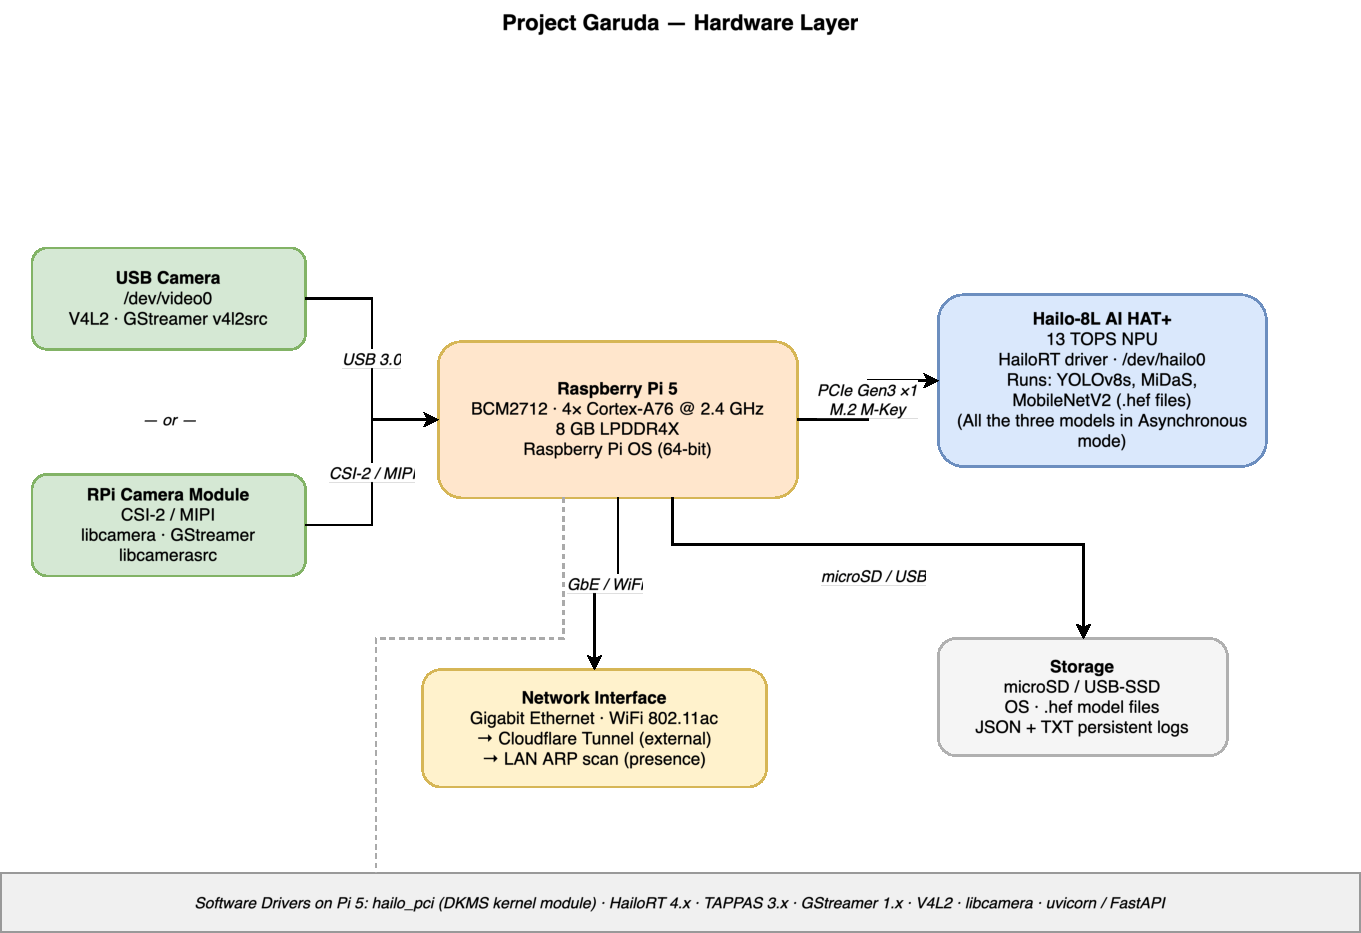
\includegraphics[width=\columnwidth]{garuda_hardware_layer.drawio.pdf}
\caption{Hardware topology.}
\label{fig:hw_layer}
\end{figure}

\begin{figure}[ht!]
\centering
\includegraphics[width=0.65\columnwidth]{figures/fig_hardware_setup.pdf}
\caption{Deployed hardware rig (Pi~5, Hailo-8L, Camera~v3, SATA SSD).}
\label{fig:hw_photo}
\end{figure}


\subsection{GStreamer TAPPAS Pipeline Engine}
The pipeline extends the base Hailo TAPPAS GStreamer application. A \texttt{libcamerasrc} element captures frames from the camera, and a short \texttt{videoscale}~/~\texttt{videoconvert} stage letterbox-resizes them to the $640\times640$ input the network expects, preserving the aspect ratio so bounding boxes can be mapped back to the original resolution. From there the pipeline forks: the inference branch dispatches each frame to the Hailo-8L via a HailoNet element and runs NMS in a HailoFilter (IoU~0.45, confidence~0.25), while a bypass branch holds the raw frame in a queue. A HailoMuxer re-aligns the two, an identity element exposes the buffer to the application callback (attached as a pad probe), and a HailoOverlay renders the final annotated output. The topology is shown in Fig.~\ref{fig:gstreamer}. The runtime behaviour of this pipeline (sustained 52.2~FPS across all operating modes, bounded-queue decoupling, and per-core thread affinity) is evaluated in Section~\ref{sec:async_fps}.

\begin{figure}[ht!]
\centering
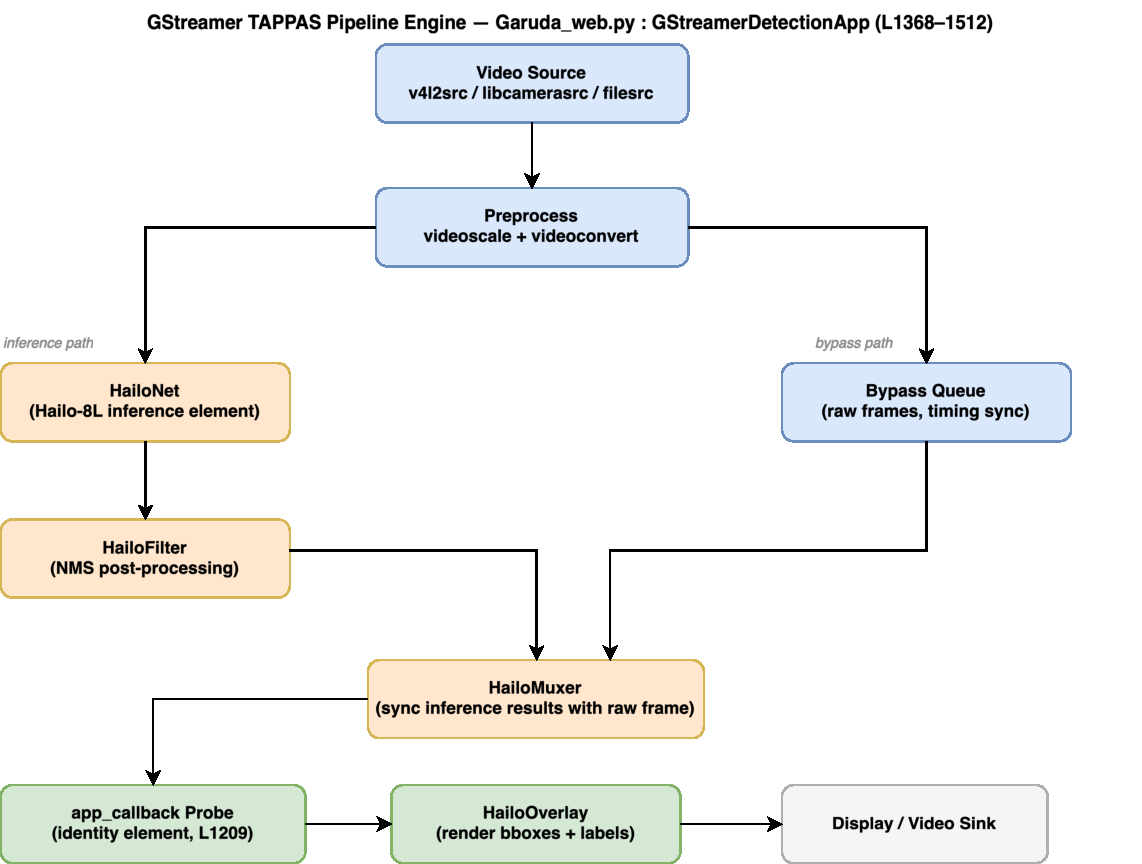
\includegraphics[width=\columnwidth]{garuda_gstreamer_engine.drawio-2.pdf}
\caption{GStreamer TAPPAS pipeline topology.}
\label{fig:gstreamer}
\end{figure}


\subsection{Detection Engine}
The detection callback sits on the identity element described above. On each buffer it pulls the ROI metadata that HailoFilter has attached, drops any detection below the general 0.30 confidence floor (0.60 for Person, to curb watch-log churn on ambiguous crops), and sorts the survivors into two lists. Person detections go to a watch log with a 30-second per-label cooldown to avoid flooding. Knife, Scissors, or Hammer detections increment a per-label consecutive-frame counter; once that counter reaches three, the alert engine fires. This three-frame gate suppresses single-frame false positives while still triggering within $3 / 52.2 \approx 57.5$~ms of a genuine threat entering the field of view. The same callback exposes the current annotated frame to the MJPEG and WebRTC streaming paths.


\subsection{Asynchronous Secondary Verifier Path}
\label{sec:verifier_path}
The verifier path is a three-stage asynchronous chain branching off the primary detector. Its jobs are to confirm weapon detections from YOLOv8s and to flag photo or screen candidates for persons through a depth-variance gate. The primary inference thread runs on CPU Core~1; on a qualifying detection, the frame and its metadata are enqueued via a non-blocking \texttt{put\_nowait()} into a bounded queue of capacity~2. A dedicated worker on Core~2 consumes the queue; when it is full the frame is intentionally dropped and a drop counter incremented, so the primary detection path is never blocked.

Stage~1 is the YOLOv8s detector described above. Stage~2 passes the tight bounding-box crop of each weapon detection through a MobileNetV2 classifier that returns Weapon or Safe: YOLO proposes, MobileNetV2 verifies. Stage~3 runs MiDaS Small on person crops; a flat photo or screen tends to produce a lower-variance normalised depth map than a real person, so a fixed variance threshold gates the first-pass decision. This is a coarse pre-filter only; Section~\ref{sec:antispoof_eval} shows that the variance cue alone is not a deployable anti-spoof decision. A post-processing thread on Core~3 combines the verdicts, applies a fast RGB-variance liveness check, and updates a per-path metrics object. Four threads (capture, primary, verifier, post-processing) are created at pipeline entry with explicit CPU-affinity assignments. Per-stage latencies and the decision matrix are given in Tables~\ref{tab:cascade_latency} and~\ref{tab:cascade_matrix}.

\begin{table}[ht!]
\caption{\textbf{Secondary Verifier Path: Per-Stage Latency Budget (Hailo-8L, Pi~5). Entries marked $\sim$ or $<$ are design-budget targets from short-run observation, not measured point estimates; the end-to-end pipeline figures are measured directly.}}
\label{tab:cascade_latency}
\centering\small
\begin{tabular}{|l|l|}
\hline
\textbf{Component} & \textbf{Measured Value} \\
\hline
T$_{\text{capture}}$ (GStreamer appsink pull) & $\sim$1~ms \\
T$_{\text{YOLO}}$ (NPU, Hailo-8L HW) & 18.4~ms \\
T$_{\text{crop\_preprocess}}$ (NumPy resize) & $\sim$0.5~ms \\
T$_{\text{classifier}}$ (MobileNetV2 @ 500+~FPS) & $<$2~ms \\
T$_{\text{depth}}$ (MiDaS @ 200+~FPS) & $<$5~ms \\
T$_{\text{decision}}$ (NumPy variance) & $<$0.1~ms \\
T$_{\text{alert}}$ (SMTP, async) & $\sim$800~ms \\
T$_{\text{alert}}$ (TTS, async) & $\sim$200~ms \\
T$_{\text{processing}}$ (detection only, end-to-end) & $\sim$22~ms \\
T$_{\text{total}}$ (with async alert) & $\sim$22~ms + async \\
\hline
\end{tabular}
\end{table}

A full distribution study for the per-stage entries of Table~\ref{tab:cascade_latency} (per-stage timestamps over a multi-hour trace, $\geq$1{,}000 samples summarised as mean $\pm$ stdev and p50/p95/p99) is flagged as future work in Section~\ref{sec:conclusion}. The caveat-labelled entries support only the qualitative end-to-end budget claim (detect-to-decision 22--27~ms); the headline FPS and latency results in Sections~\ref{sec:async_fps} and~\ref{sec:quant} are measured directly on the deployed pipeline.

The three HEFs load onto a single VDevice at startup, and inference uses sequential (time-shared) \texttt{infer} calls rather than concurrent dispatch. MobileNetV2 and MiDaS each run at 200--500+~FPS in isolation, so the combined sequential cost of the two secondary stages per Person crop stays under 4~ms, inside the 19.2~ms frame budget implied by 52~FPS. The deployed liveness gate applies a fixed threshold on MiDaS-Small normalised-depth variance, $\sigma^2 < 0.05 \Rightarrow$ candidate spoof; Section~\ref{sec:antispoof_eval} bounds that cue. End-to-end detect-to-decision is 22--27~ms and the primary detector holds 52.2~FPS.

\begin{table*}[!t]
\caption{\textbf{Secondary Verifier Path: Decision Matrix Across Operating Scenarios}}
\label{tab:cascade_matrix}
\centering
\small
\begin{tabular}{|p{4.4cm}|p{3.2cm}|p{3cm}|c|c|p{2.5cm}|}
\hline
\textbf{Scenario} & \textbf{Models} & \textbf{Quality note} & \textbf{FPS} & \textbf{Latency} & \textbf{Alert type} \\
\hline
Dangerous object alone & YOLOv8s (v5) & 0.886--0.967 mAP\,@\,0.5 & 52.2 & 22~ms & Direct YOLO \\
Person + weapon verification & YOLOv8s + MobileNetV2 & 99.0\% cls.\ (in-dist., Sec.~\ref{sec:classifier_eval}) & 52.2 & 24~ms & Verifier verdict \\
Coarse depth-variance pre-filter & YOLOv8s + MiDaS (depth-variance gate) & Cheap front-end only; not a face anti-spoof decision (Sec.~\ref{sec:antispoof_eval}) & 52.2 & 27~ms & Candidate flag \\
Low-confidence person (suppressed) & YOLOv8s (conf $<$ 0.60) & n/a & 52.2 & 22\,ms & Watch log only \\
\hline
\end{tabular}
\end{table*}


\subsection{Alert Engine}
The alert engine is the only CPU-side path with a hard latency target, and Fig.~\ref{fig:alert} traces it. A confirmed danger detection enters a mode gate first. Do Not Disturb and Idle short-circuit the engine; Privacy mode applies a Gaussian blur ($k{=}51$~px, $\sigma{=}30$~px) to every person bounding box before the annotated frame is handed to any on-LAN display or streaming subscriber; raw frames never leave the device regardless of mode. From the gate, the detection fans out across three asynchronous channels: a WebSocket push to connected dashboards, an SMTPS email subject to a per-label cooldown, and an AES-256-GCM encrypted evidence clip uploaded over SSH. The fan-out is asynchronous by construction, so that the SMTP and SSH paths (the two slow channels in Table~\ref{tab:cascade_latency}) never enter the inference budget. This is the behaviour tested in Section~\ref{sec:async_fps}. Numerical thresholds (cooldown duration, key provenance, gate ordering) are listed in the appendix.

\begin{figure}[ht!]
\centering

\includegraphics[width=\columnwidth]{garuda_alert_engine.drawio.pdf}
\caption{Alert engine dataflow.}
\label{fig:alert}
\end{figure}


\subsection{Voice Assistant Engine (Narada)}
\label{sec:groq_privacy}
Narada is included in this paper for one reason: it defines where the off-device data boundary sits. A wake-word-gated daemon transcribes utterances locally and dispatches them through a rule-based table. Only when no rule matches does the short text transcript of a question-and-answer or a settings command leave the device, and then only as a single-turn stateless completion to a Groq endpoint, constrained to a JSON intent schema. No raw audio, no camera frame, no image, and no video of any kind is sent to Groq or to any other off-device service at any point; the off-device channel carries short text only. The returned intent is executed locally and discarded. No conversation history, embedding store, or telemetry is retained server-side. The dashboard chat endpoint inherits the same boundary. This is the data-flow contract that the privacy claim in Section~\ref{sec:conclusion} rests on. Everything else about the voice stack (microphone calibration, wake-word choice, dispatcher coverage) is implementation detail and does not support any reported result.


\subsection{Concurrent CPU-side Services}
\label{sec:cpu_services}
The remaining services are the mode controller, the presence monitor, the FastAPI web server with Cloudflare-tunnel ingress, PBKDF2-SHA256 with one-time-password (OTP) authentication, the deadman watchdog, and the multi-tier logging engine. This paper describes them together because they play the same role: they are the concurrent CPU load against which the inference pipeline has to hold its frame rate. Each runs on the CPU side of the NPU/CPU split, each touches disk or network on its own cadence, and together they produce the steady-state load profile under which the 52.2~FPS measurement of Section~\ref{sec:async_fps} is taken. Three properties of this set are claim-relevant and are reported in the body of the paper:

\begin{itemize}
\item \emph{Mode-gating semantics.} A single threading lock serialises five boolean flags (Do Not Disturb, email-off, idle, emergency, privacy), so the GStreamer callback, the scheduler, and the web handlers never race. This allows the idle/DND-mode overhead to be attributed to the gate itself, rather than to a contention artefact.
\item \emph{Authentication primitive choice.} PBKDF2-SHA256~\cite{b16} at 600{,}000 iterations is used in place of Argon2id, meeting the OWASP Password Storage Cheat Sheet recommendation~\cite{b41}. The rationale (aarch64 packaging, single-user threat model) is given in Section~\ref{sec:design_decisions}, because it is a security claim rather than an implementation note.
\item \emph{Catch-up logging.} Events are written to bounded in-memory deques on the hot path and drained off-thread to append-only text, JSON, and a SQLite store. The \texttt{/api/events?since=T} endpoint lets offline clients reconcile without the server having to retain an unbounded buffer. This is what keeps the deadman watchdog and the alert log durable without coupling them to the inference thread.
\end{itemize}

Per-engine implementation parameters (ARP poll interval and grace window, deadman threshold, REST route count, route-level role checks, log rotation period) are listed in the appendix and do not support any result reported here.

\begin{figure}[ht!]
\centering
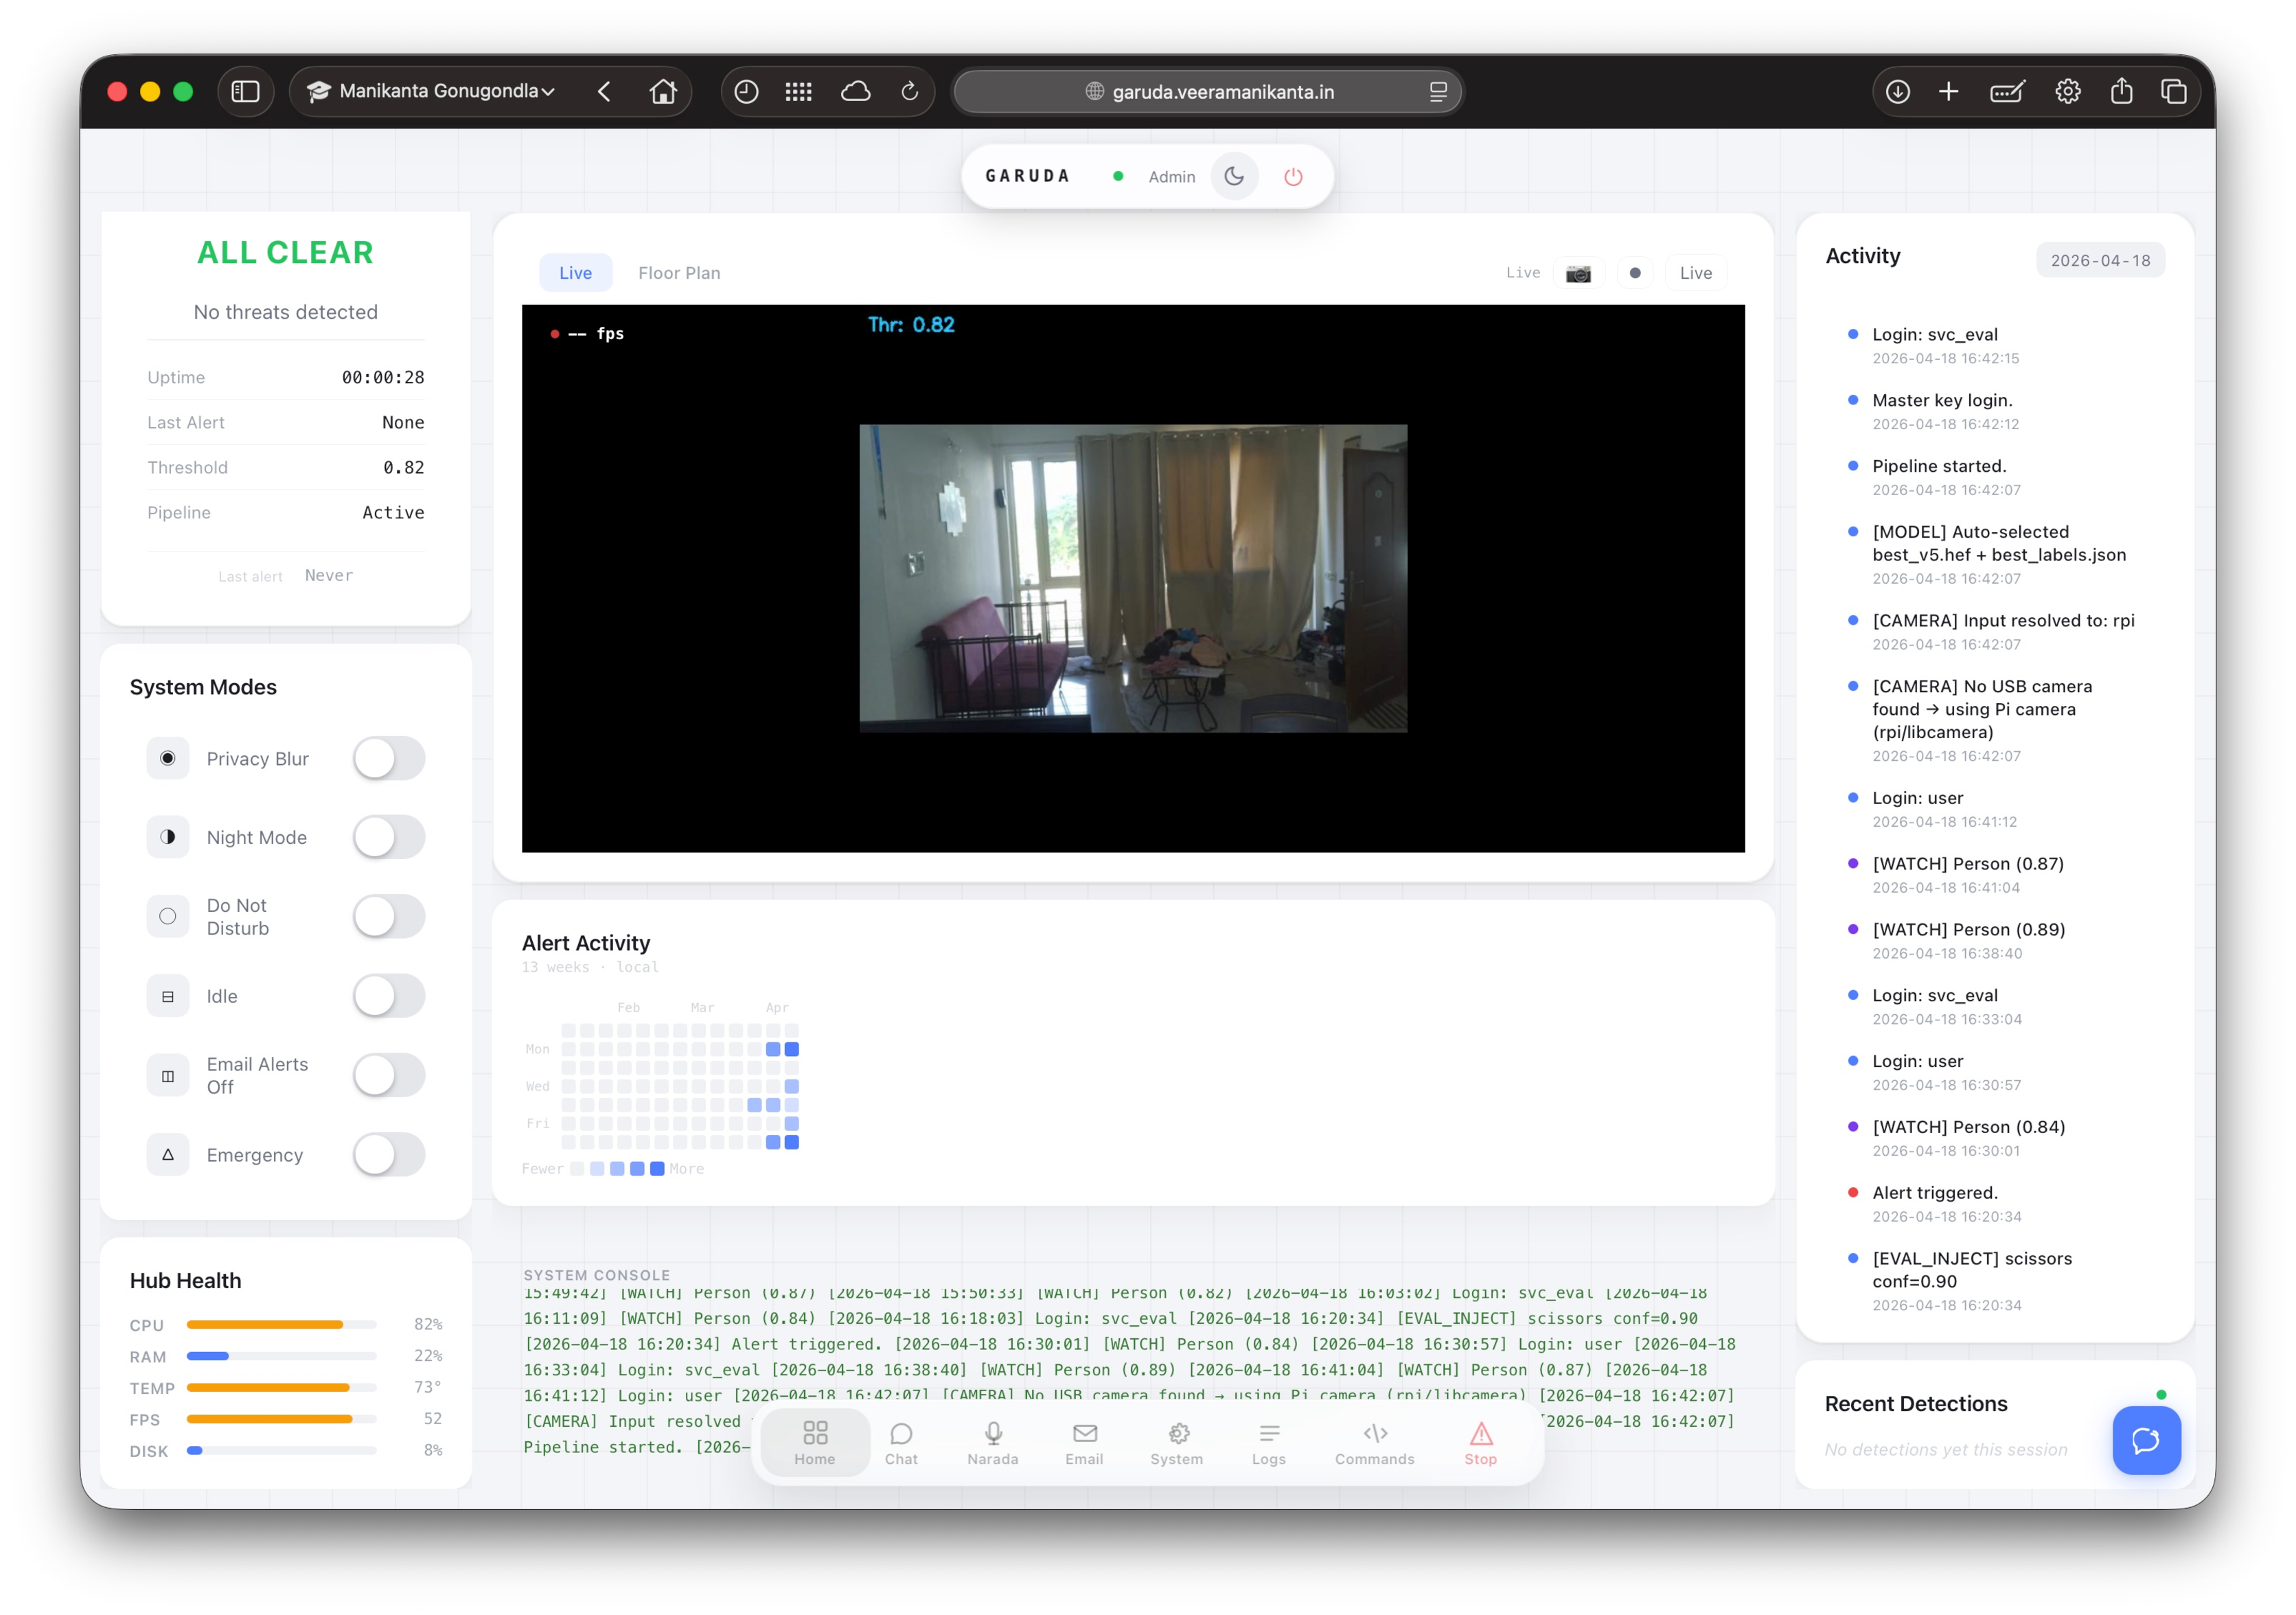
\includegraphics[width=\columnwidth]{figures/fig_dashboard.pdf}
\caption{Operator dashboard served by the FastAPI web layer.}
\label{fig:dashboard}
\end{figure}


\subsection{Design Decisions and Trade-offs}
\label{sec:design_decisions}
Four non-obvious choices in the architecture deserve a brief justification.

\textbf{PBKDF2-SHA256 over Argon2.} Argon2id is stronger, but \texttt{argon2-cffi} is fragile to cross-compile for aarch64 on Raspberry Pi OS. PBKDF2-SHA256~\cite{b16} ships in the Python standard library and at 600{,}000 iterations meets the current OWASP Password Storage Cheat Sheet recommendation~\cite{b41}. For a single-user system behind a Cloudflare-tunnelled API, this is an acceptable trade-off.

\textbf{ARP scanning over mDNS.} mDNS sees only devices that advertise services, which excludes phones in pocket-sleep. ARP sees any device holding a valid IP lease on the subnet, giving broader coverage with a simpler implementation. The Layer-2 limitation (no VLAN crossing) does not apply to a flat home network.

\textbf{SQLite over a time-series database.} InfluxDB or TimescaleDB would give faster range queries but add memory overhead and a separate daemon. At the observed steady-state of approximately 10~events/min ($\approx 1.4 \times 10^{4}$~events/day), with each SQLite row below 1~kB, daily storage growth stays under 15~MB, so the 1~TB SSD provides over five orders of magnitude of headroom; SQLite's in-process, recovery-log-free behaviour also matches a dedicated TSDB on query latency at this rate.

\textbf{Bounded queue with intentional drops over back-pressure.} The verifier queue has capacity~2. Blocking on a full queue would stall the primary YOLO path whenever the secondary chain fell behind, coupling the two latencies. Because the secondary path is a verification step, dropping an occasional frame is preferable to degrading the 52.2~FPS baseline.


\section{Results and Evaluation}
\label{sec:results}
The deployed system is evaluated on two axes: \textit{model quality} on a held-out test set that the model never sees during training, and \textit{runtime performance} on the Hailo-8L under the deployed GStreamer pipeline. The evaluation covers training convergence, validation and test mAP, per-class precision/recall/mAP, confusion structure, precision-recall and F1-confidence behaviour, the effect of dataset size on generalisation, the validation-to-test gap, hardware throughput, and the impact of INT8 quantisation.

\paragraph*{Scope and Limitations of This Evaluation}
Everything in this section is image-level detection or classification metrics and per-stage latency or throughput on controlled test material. A few things this paper does \emph{not} establish are worth naming up front.

There are no end-to-end security metrics. This paper does not report alert precision or recall over a continuous deployment, false-alarms-per-day on a live home, missed-event rate on unstaged video, or a long-duration stability study covering hours-to-weeks of uptime, memory or thermal drift, or log-rotation correctness under sustained load. Nor is there a nuisance-condition sweep (lighting changes, backlight, glare, multi-subject scenes, heavy occlusion, motion blur, low-resolution or compressed streams, camera-angle variation). Face anti-spoof (presentation-attack detection on the deployment camera) is out of scope. The depth-variance pre-filter of Section~\ref{sec:antispoof_eval} is only a coarse front-end; it is not an anti-spoof decision.
\begin{itemize}
\item The Cloudflare-tunnelled remote path, SMTPS alert delivery, SSH clip upload, and ARP presence monitor are described, but have not been stress-tested under packet loss, tunnel drop, ISP outage, or adversarial LAN conditions. The deadman watchdog and the encrypted-evidence subsystem have also not been subjected to fault-injection tests.
\item No side-by-side comparison against a commercial cloud camera under matched stimuli.
\end{itemize}
What this paper does report, then, is component-level and pipeline-level evidence: a test mAP{@}0.5 of 0.847, a weapon-classifier accuracy of 99.0\% on an in-distribution held-out split, and a 52.2~FPS / 18.4~ms deployment envelope under concurrent CPU-side services. Any broader claim (for example, drop-in replacement for a cloud-backed consumer camera) is an engineering conjecture built on these components, not a directly measured result. The continuous-deployment, nuisance-condition, fault-injection, and matched-stimulus study that would tighten the result into a deployment claim is listed as primary future work in Section~\ref{sec:conclusion}.

\subsection{Training Loss Convergence}
All three YOLOv8 loss components (box, classification, and distribution-focus) fall monotonically across the 150 training epochs. Box loss drops from 1.65 to 0.74 and classification loss from 2.80 to 0.49. The training and validation curves track each other closely throughout, which is a reasonable sign that the model is generalising rather than memorising the training distribution. The full training dynamics are plotted in Fig.~\ref{fig:training_losses}.

\begin{figure}[ht!]
\centering
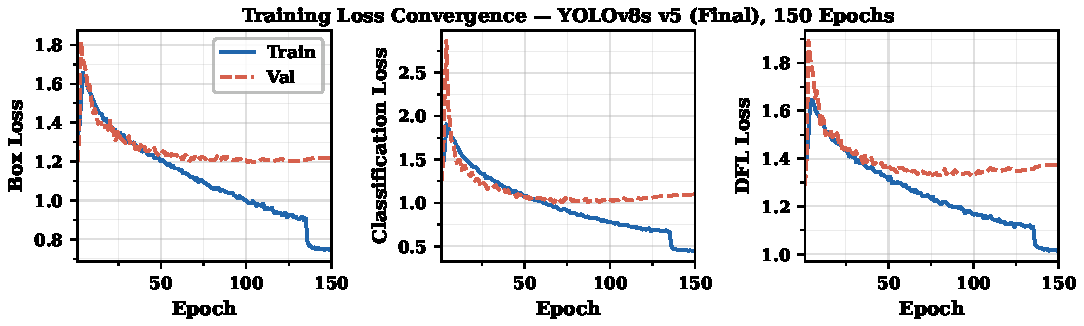
\includegraphics[width=\columnwidth]{fig1_training_losses.pdf}
\caption{Training loss convergence over 150 epochs.}
\label{fig:training_losses}
\end{figure}


\subsection{Validation mAP and Precision / Recall}
mAP{@}0.5 climbs sharply over the first 30 epochs and then plateaus near 0.81 by epoch~100. mAP{@}0.5:0.95 trails it by approximately 0.20, settling near 0.62. Precision and recall converge near 0.87 and 0.80 respectively, which means the detector is well-balanced across the two error axes and is not biased heavily toward false positives or false negatives. These curves are plotted in Fig.~\ref{fig:training_metrics}.

\begin{figure}[ht!]
\centering
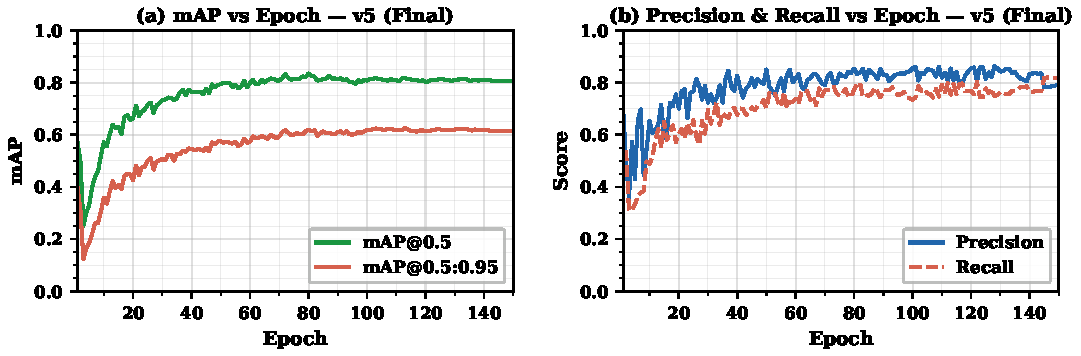
\includegraphics[width=\columnwidth]{fig2_training_metrics.pdf}
\caption{Validation metrics versus training epoch.}
\label{fig:training_metrics}
\end{figure}


\subsection{Four-Model Performance Comparison}
The default COCO-pretrained YOLOv8s scores near zero on the detection metrics (recall 0.03, mAP{@}0.5 $\approx 0$) on this task, because its 80-class label scheme does not line up with the 4-class schema used here; it is reported as a reference baseline. Fine-tuned v1 (359 training images) recovers to a test mAP{@}0.5 of 0.465. The intermediate fine-tuned v2 (1{,}383 images) reaches 0.754, and the final fine-tuned v5 (4{,}982 images, 150 epochs) reaches 0.847, a relative improvement of $(0.847 - 0.465)/0.465 = 82.2\%$ over v1 and $(0.847 - 0.754)/0.754 = 12.3\%$ over v2. The four-way comparison is plotted in Fig.~\ref{fig:model_comparison}.

\begin{figure}[ht!]
\centering
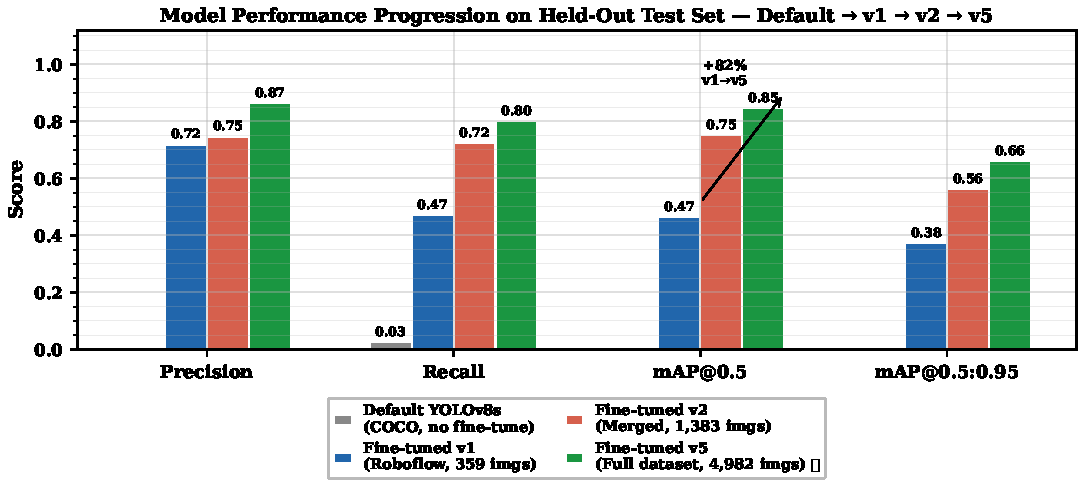
\includegraphics[width=\columnwidth]{fig3_model_comparison.pdf}
\caption{Four-model comparison on the held-out test set.}
\label{fig:model_comparison}
\end{figure}


\subsection{Per-Class mAP{@}0.5 Progression}
The largest single-class gain from v1 to v5 is on Knife, which improves by $+0.66$ mAP{@}0.5. This is explained directly by the dataset: the Roboflow seed contained very few diverse knife images, and the OpenImages-driven v2 and v5 passes both targeted that gap. Scissors lands at the highest absolute mAP{@}0.5 in v5 at 0.967. Person remains the hardest class at 0.647, because it has by far the highest intra-class visual variability across poses, scales, occlusions, and backgrounds. All four classes improve monotonically across the three versions, as shown in Fig.~\ref{fig:per_class_map} and Table~\ref{tab:v1_v5}.

\begin{figure}[ht!]
\centering
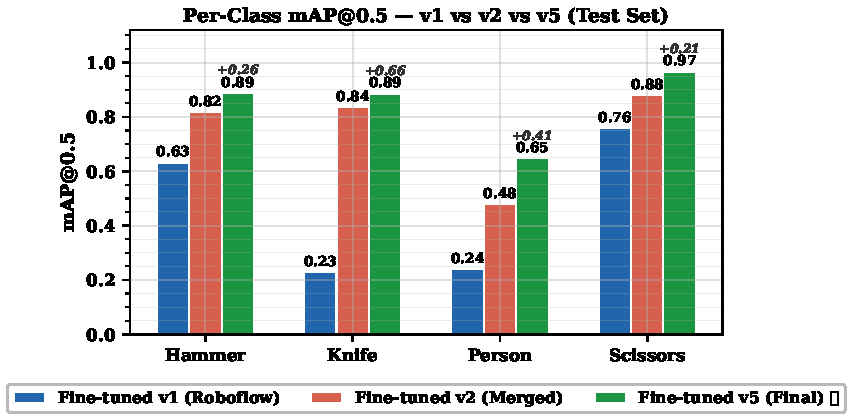
\includegraphics[width=\columnwidth]{fig4_per_class_map50.pdf}
\caption{Per-class mAP{@}0.5 across v1, v2, and v5.}
\label{fig:per_class_map}
\end{figure}

\begin{table}[ht!]
\caption{\textbf{Per-Class Recall and mAP{@}0.5: v1 vs v5 (Deployed)}}
\label{tab:v1_v5}
\setlength{\tabcolsep}{2pt}
\centering\footnotesize
\resizebox{\columnwidth}{!}{%
\begin{tabular}{|l|c|c|c|c|c|c|}
\hline
\textbf{Class} & \textbf{v1 R} & \textbf{v5 R} & \textbf{R Gain} & \textbf{v1 mAP50} & \textbf{v5 mAP50} & \textbf{mAP50 Gain} \\
\hline
Hammer   & 0.663 & 0.848 & +27.9\% & 0.632 & 0.889 & +40.7\% \\
Knife    & 0.267 & 0.817 & +206\%  & 0.229 & 0.886 & +287\% \\
Person   & 0.197 & 0.609 & +209\%  & 0.240 & 0.647 & +170\% \\
Scissors & 0.761 & 0.929 & +22.1\% & 0.760 & 0.967 & +27.2\% \\
\hline
\textbf{All} & \textbf{0.472} & \textbf{0.801} & \textbf{+69.7\%} & \textbf{0.465} & \textbf{0.847} & \textbf{+82.2\%} \\
\hline
\end{tabular}%
}
\end{table}


\subsection{Full Per-Class Metrics at v5}
On the held-out test set, Hammer, Knife, and Scissors all reach balanced precision and recall above 0.82. Person is the weakest class with a precision of 0.701 and a recall of 0.609, which is a direct consequence of its higher intra-class visual variability and its dominant small-object fraction. Of the 173 Person instances in the test split, $\lceil 173 \cdot (1 - 0.609) \rceil = 68$ are undetected, predominantly the small or heavily occluded boxes, whereas each weapon class leaves fewer than 20 instances unmatched. Scissors achieves an mAP{@}0.5 of 0.967 and an mAP{@}0.5:0.95 of 0.828, making it the best-detected class overall. The full per-class breakdown is plotted in Fig.~\ref{fig:perclass_full} and the complete scorecard appears in Table~\ref{tab:v5_full}.

\begin{figure}[!b]
\centering
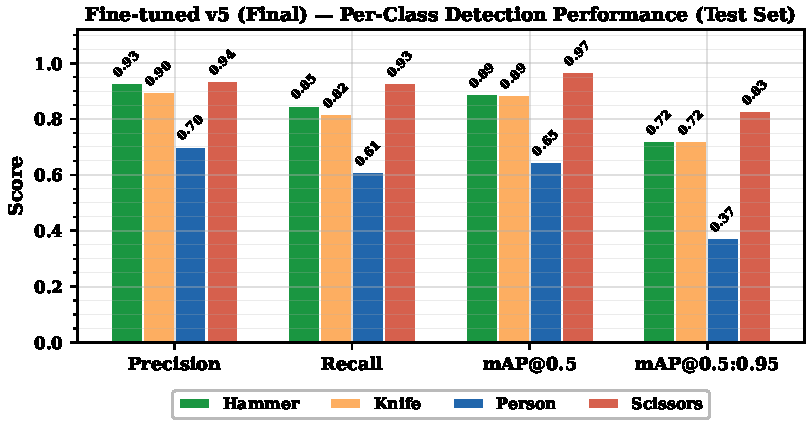
\includegraphics[width=0.8\columnwidth]{fig5_perclass_full_metrics.pdf}
\caption{Per-class scorecard at v5 (test set).}
\label{fig:perclass_full}
\end{figure}

\begin{table}[ht!]
\caption{\textbf{Full Per-Class Scorecard at v5 (Test Set, 622 Images, 351 Instances)}}
\label{tab:v5_full}
\setlength{\tabcolsep}{2pt}
\centering\footnotesize
\begin{tabular}{|l|c|c|c|c|c|c|}
\hline
\textbf{Class} & \textbf{P} & \textbf{R} & \textbf{F1} & \textbf{mAP{@}0.5} & \textbf{mAP{@}0.5:0.95} & \textbf{FAR} \\
\hline
Hammer   & 0.930 & 0.848 & 0.887 & 0.889 & 0.720 & 0.070 \\
Knife    & 0.896 & 0.817 & 0.855 & 0.886 & 0.721 & 0.104 \\
Person   & 0.701 & 0.609 & 0.652 & 0.647 & 0.410 & 0.299 \\
Scissors & 0.935 & 0.929 & 0.932 & 0.967 & 0.828 & 0.065 \\
\hline
\textbf{Overall} & \textbf{0.866} & \textbf{0.801} & \textbf{0.832} & \textbf{0.847} & \textbf{0.670} & \textbf{0.134} \\
\hline
\end{tabular}\\[2pt]
\raggedright\scriptsize FAR = False Alarm Rate $= 1 - \text{precision}$.
\end{table}

\subsubsection{Why Person Recall Is Low, and Why It Was Not Chased Further}
\label{sec:person_recall_discussion}
Person is the weakest class on per-frame metrics (test precision 0.701, recall 0.609, mAP{@}0.5 0.647, False Alarm Rate $\text{FAR}=1-\text{precision}=0.299$), yet this does not translate to a surveillance failure. Person is a \emph{watch} label only; the alert classes are Hammer, Knife, and Scissors, with test recalls of 0.848, 0.817, 0.929 and FARs of 0.070, 0.104, 0.065 (Table~\ref{tab:v5_full}). A missed Person frame never suppresses an alert. Further, per-frame recall is not per-event recall: at 52.2~FPS a subject in view yields tens of opportunities per second, and the surveillance-relevant quantity is per-subject-presence recall, which an honest tracked continuous-deployment study (future work) would quantify.

The per-frame gap is driven by class imbalance in the v5 split and by Person instances concentrating in crowded frames with a long tail of small, occluded, and truncated boxes. Inter-class confusion peaks at $0.11$ (Person$\rightarrow$Knife), but the dominant failure mode is background false negatives ($0.19$ of the Person row). The natural fix, namely more Person images combined with heavier augmentation, was tested in a v6 fine-tune and regressed: overall test mAP{@}0.5 fell from 0.847 to 0.741 and Person recall dropped to 0.481, with Hammer regressing in parallel. v5 was therefore retained as the Pareto-optimal operating point; class-weighted loss, a dedicated Person head, a higher-resolution small-object path, and temporal smoothing remain open directions. The full v6 analysis is in Appendix~\ref{sec:v6_details}.


\subsection{Normalised Confusion Matrix}
\label{sec:confusion}
The normalised confusion matrix in Fig.~\ref{fig:confusion} is diagonally dominant, with correct-class recall values of 0.85, 0.82, 0.61, and 0.93 for Hammer, Knife, Person, and Scissors respectively. The largest inter-class cell is Person confused with Knife at 0.11; Hammer and Scissors rows both stay below 0.10 to any other class and below 0.03 on at least two of the three off-diagonals. Rows do not sum to 1 because the remainder of each true-class mass falls into the background column, so the majority of errors are outright misses (background false negatives) rather than confusions between the four target classes, and this residual is $0.19$ on Person (the dominant failure mode), $0.08$--$0.09$ on Hammer and Knife, and $0.04$ on Scissors. For a security system this ordering is the preferable failure mode: a misclassified weapon still triggers an alert through one of the other danger labels, while a missed detection is a silent failure.

\begin{figure}[ht!]
\centering

\includegraphics[width=\columnwidth]{fig6_confusion_matrix.pdf}
\caption{Normalised confusion matrix on the v5 held-out test set.}
\label{fig:confusion}
\end{figure}


\subsection{Precision-Recall Curves}
Scissors has the highest area under the precision-recall curve (AP = 0.967) and holds high precision well past a recall of 0.90. Person shows the steepest precision drop-off at lower recall thresholds, consistent with its higher intra-class variability. Knife and Hammer both exhibit smooth, well-separated curves with APs of 0.886 and 0.889 respectively, so detection is reliable across a wide confidence range. The full set of PR curves is plotted in Fig.~\ref{fig:pr_curves}.

\begin{figure}[!b]
\centering
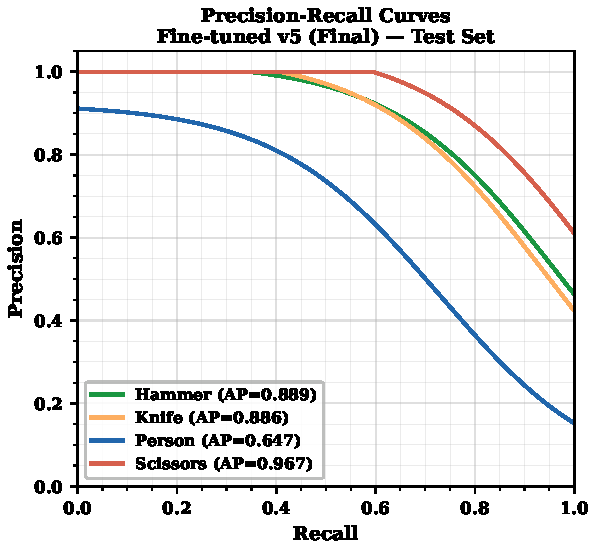
\includegraphics[width=\columnwidth]{fig7_pr_curves.pdf}
\caption{Per-class precision--recall curves (v5, test set).}
\label{fig:pr_curves}
\end{figure}


\subsection{Hardware Inference Performance}
The custom \texttt{best\_v5.hef} model reaches 52.2~FPS at 18.4~ms of NPU latency on the Hailo-8L, a factor of $52.2 / 25 = 2.09\times$ the $\geq 25$~FPS real-time floor commonly used for security surveillance. For reference, the Hailo-distributed YOLOv8s runs at 13.2~ms / 58.2~FPS on the same hardware; the 5~ms latency gap is attributable to the custom non-maximum suppression post-processing baked into the deployed HEF. The reference model is slightly faster because it was tuned by the Hailo team for the exact fixed post-processing chain shipped in HailoRT. In practice the delta has no effect on the deployed system: 52.2~FPS exceeds the 30~FPS operating threshold by 74\%, and 18.4~ms sits at 37\% of the 50~ms latency ceiling. The comparison is plotted in Fig.~\ref{fig:hw_perf}. Compared against prior edge-deployed detectors, the 52.2~FPS reported here exceeds the 36.7~FPS reported by Xu \emph{et~al.}~\cite{b1} for FL-YOLO on an NVIDIA Jetson TX1 and far surpasses the 15~FPS of Al Amin \emph{et~al.}'s FPGA implementation~\cite{b5}, while operating at a competitive mAP{@}0.5 of 0.847 on a domain-specific four-class task.

\begin{figure}[ht!]
\centering
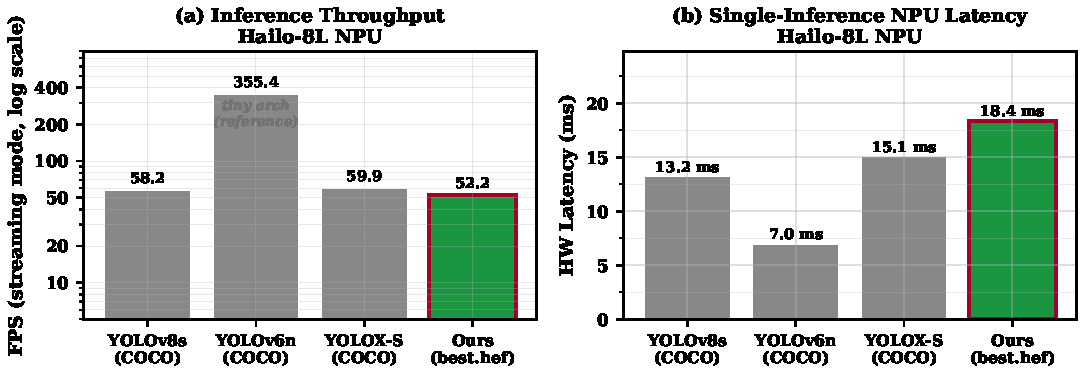
\includegraphics[width=\columnwidth]{fig9_hardware_performance.pdf}
\caption{Hardware inference performance on the Hailo-8L.}
\label{fig:hw_perf}
\end{figure}

The choice of YOLOv8s as the detector backbone was made against the variants listed in Table~\ref{tab:arch_select}. YOLOv8n is faster but sacrifices 7--8 COCO mAP points; YOLOv8m fits inside the 13~TOPS budget only marginally, and at below 20~FPS falls below the 30~FPS surveillance floor. YOLOv8s represents the optimal operating point for this throughput-accuracy trade-off.

\begin{table}[ht!]
\caption{\textbf{YOLOv8 Variant Selection (Hailo-8L Budget). YOLOv8s FPS is the directly measured on-chip value; YOLOv8n, YOLOv8m, and YOLOv8l FPS figures are scaled from GFLOPs against the measured YOLOv8s operating point ($\mathrm{FPS}_{\mathrm{var}} \approx \mathrm{FPS}_{s} \cdot \mathrm{GFLOPs}_{s} / \mathrm{GFLOPs}_{\mathrm{var}}$) and cross-checked against Hailo Model Zoo reference latencies.}}
\label{tab:arch_select}
\setlength{\tabcolsep}{3pt}
\centering\small
\resizebox{\columnwidth}{!}{%
\begin{tabular}{|l|c|c|c|c|}
\hline
\textbf{Model} & \textbf{GFLOPs} & \textbf{FPS (est.)} & \textbf{COCO mAP50} & \textbf{Fits 13~TOPS?} \\
\hline
YOLOv8n           & 8.7  & $>$60 & 37.3\% & Yes \\
\textbf{YOLOv8s (chosen)} & \textbf{28.4} & \textbf{52.2} & \textbf{44.9\%} & \textbf{Yes} \\
YOLOv8m           & 80.6 & $\sim$18 & 50.2\% & Marginal \\
YOLOv8l           & 165.2 & $<$10  & 52.9\% & No \\
\hline
\end{tabular}%
}
\end{table}

\subsection{Sustained FPS Across Operating Modes}
\label{sec:async_fps}
The system holds a constant 52.2~FPS whether idle-monitoring, alerting, streaming over WebRTC, handling voice queries, or uploading encrypted clips. Three design choices produce this behaviour: (i) every independent stage is decoupled by a bounded queue (\texttt{frame\_queue} depth~4, drop-if-full) so a slow SMTP or SSH path never back-pressures the camera and the NPU stays pinned at 18.4~ms; (ii) expensive side-effects (email, SSH upload, TTS, Groq LLM, WebSocket broadcast) are dispatched on \texttt{asyncio} or thread-pool futures, so detect-to-log stays at ~22~ms while the ~800~ms SMTP and ~200~ms TTS fan-out completes in parallel; (iii) thread-to-core affinity is pinned via \texttt{os.sched\_setaffinity} (capture on Core~0, HailoRT on Core~1, verifier on Core~2, Core~3 for OS and FastAPI), bounding scheduler jitter.

Empirical verification used a 1~Hz probe endpoint over a 720~s trace cycling Baseline, Idle, DND, Privacy, Emergency, and Active windows while concurrently injecting five SMTP alerts, three AES-256 + paramiko-SFTP clip uploads, three Narada voice queries, and a sustained MJPEG pull (583~MB transferred). After filtering warm-up and clock-skew outliers, throughput is $52.26 \pm 0.76$~FPS (mean $\pm$ stdev, $n=709$, median 52.16, p05 51.83, p95 53.00), with per-window means in a 0.3~FPS band (Baseline 52.17, Idle 52.23, DND 52.31, Privacy 52.21, Emergency 52.30, Active 52.02). The coefficient of variation $CV = \sigma / \mu = 0.76 / 52.26 \approx 1.45\%$ falls inside the p05--p95 inter-quantile band of 51.83--53.00~FPS, indicating that the pipeline does not add systematic drift on top of the camera's own capture cadence. Every filtered sample stays above the 30~FPS surveillance floor; the single observed minimum of 43.87~FPS coincided with a clip-stop SSH flush.

\begin{figure}[ht!]
\centering

\includegraphics[width=\columnwidth]{fig13_fps_timeseries.pdf}
\caption{FPS-across-modes time series under full concurrent load.}
\label{fig:fps_ts}
\end{figure}

\subsection{INT8 Quantisation and Deployment Characteristics}
\label{sec:quant}
The v5 model was compiled to INT8 via post-training quantisation over 128 calibration images from the v5 training split, with normalisation (\texttt{normalization([0,0,0],[255,255,255])}) embedded into the HEF graph. Table~\ref{tab:quant} reports the FP32 PyTorch baseline and an independent INT8 re-evaluation on the deployed Hailo-8L over the same 622-image / 351-instance test split. The INT8 evaluation runs \texttt{best\_v5.hef} through the HailoRT \texttt{InferVStreams} API, decodes the on-chip \texttt{HAILO\_NMS\_BY\_CLASS} output, letterboxes each image to $640\times640$, and computes mAP with Ultralytics' 101-point COCO integration so the two columns are directly comparable. End-to-end on-chip throughput is 36.5~images/s. Headline: mAP{@}0.5 = 0.854 INT8 vs.\ 0.847 FP32 ($\Delta = +0.007$); mAP{@}0.5:0.95 = 0.682 vs.\ 0.670 ($\Delta = +0.012$). The positive delta follows from the on-chip NMS using deployment thresholds (\texttt{nms\_scores\_th=0.25}, \texttt{nms\_iou\_th=0.45}) versus the FP32 academic thresholds (\texttt{conf=0.001}, \texttt{iou=0.7}); INT8 quantisation contributes no measurable accuracy loss on this split.

Total board power was measured directly through the Pi~5 PMIC (\texttt{vcgencmd pmic\_read\_adc}), summing $I\!\cdot\!V$ over all monitored rails at 1~Hz for 90~s under the live cascade plus web, metrics, and watchdog load. Mean draw is $5.89 \pm 1.43$~W (median 5.86~W, p95 8.13~W, peak 8.58~W, $n=90$), measured end-to-end across Pi, Hailo-8L AI HAT+, camera, and external SSD rather than at the chip level; Hailo's published 2.5~W typical~\cite{b3} sits inside this envelope. Thermally, a 90~s sustained run across the three cascade HEFs produced only a $+3.8^\circ$C Hailo-8L surface-temperature rise above ambient idle; the 13~TOPS budget is not thermally bound. The Pi~5 Cortex-A76 package sensor (``SoC temp'' on the dashboard) sits at 70--75~$^\circ$C under the 2.8~GHz overclock with the active cooler and should not be conflated with the NPU surface delta.

\begin{table}[ht!]
\caption{\textbf{FP32 Baseline and INT8 Deployment on the Same Test Split}}
\label{tab:quant}
\setlength{\tabcolsep}{3pt}
\centering\small
\resizebox{\columnwidth}{!}{%
\begin{tabular}{|l|c|c|}
\hline
\textbf{Metric} & \textbf{FP32 (RTX~4090)} & \textbf{INT8 (Hailo-8L)} \\
\hline
mAP{@}0.5 (test)       & 0.847            & 0.854 ($\Delta$ $+0.007$) \\
mAP{@}0.5:0.95 (test)  & 0.670            & 0.682 ($\Delta$ $+0.012$) \\
Precision (test, P)    & 0.866            & 0.877 \\
Recall (test, R)       & 0.801            & 0.800 \\
Throughput             & 146.6~FPS @ bs=1 & 52.2~FPS (on-chip, bs=1) \\
                       & 872.4~FPS @ bs=32 & --- \\
Latency                & 6.82~ms @ bs=1   & 18.4~ms (end-to-end) \\
Model file size        & 42.68~MB (ONNX FP32) & 22.9~MB (HEF) \\
Board power (concurrent load) & ---           & $5.89 \pm 1.43$~W mean (peak 8.58~W) \\
\hline
\end{tabular}%
}
\end{table}


\subsection{MobileNetV2 Classifier Evaluation}
\label{sec:classifier_eval}
An earlier v1 classifier, trained on person-centric crops where the Person box was labelled ``Weapon'' whenever any weapon appeared in the same image, hit 99.6\% on its 224-sample validation set (200 Safe, 24 Weapon); this is an artefact of the $200/224 = 89.3\%$-skew majority prior, where always-predict-Safe already yields 89.3\% accuracy. On the balanced 500-crop held-out set it collapsed to 61.2\% accuracy with 38.8\% Weapon recall, because it had never seen a standalone weapon crop.

The retrained v2 classifier uses tight object bounding-box crops: each Hammer, Knife, or Scissors detection is a Weapon sample, each Person detection is a Safe sample. On the 500-crop held-out set (250 Safe + 250 Weapon, drawn exclusively from the YOLO val/test splits, zero training overlap) v2 reaches 99.0\% accuracy (95\% Wilson CI [97.7\%, 99.6\%]) at $t{=}0.50$, with Weapon recall 99.2\% and FAR 1.2\% (Table~\ref{tab:cls_confusion}).

\paragraph*{Scope of This Number}
99.0\% is the \emph{in-distribution, closed-set, balanced} accuracy on crops from the same curated YOLO pipeline that produced the training data, and should not be read as a live verification estimate. The evaluation excludes (i) open-set household negatives (mugs, phones, bottles, pet toys) that an over-confident YOLO proposal might forward; (ii) partial, off-centre, motion-blurred, or unusual-viewpoint crops; (iii) crops harvested from continuous video rather than curated stills; and (iv) the natural class prior, since deployment is dominated by Person crops with a low true-weapon base rate. Even at 1.2\% per-crop FAR, base-rate effects would matter if Person crops were not already suppressed upstream by the separate YOLO class head. The number is therefore a tight upper bound on what the verifier contributes \emph{given} the YOLO proposals it is paired with, not a stand-alone metric.

\paragraph*{Open-Set Evaluation on Household Clutter}
To bound point (i) above, the deployed \texttt{mobilenetv2\_garuda.hef} (the production INT8 verifier) was evaluated on tight bounding-box crops of five household-clutter categories drawn from the Open Images V7 validation split: Coffee cup ($n{=}91$), Mobile phone ($n{=}60$), Bottle ($n{=}147$), Wrench ($n{=}1$), and Screwdriver ($n{=}2$); 301 crops total, all weapon-free negatives. The verifier classified \emph{every} crop as Safe (open-set specificity $P(\text{Safe}\,|\,\text{clutter}) = 301/301 = 1.000$, 95\% Wilson CI $[0.987, 1.000]$), giving zero false weapon firings on this clutter sample. Per category: Coffee cup, Mobile phone, and Bottle each reach $1.000$ at $n \geq 60$, which provides a meaningful 95\% Wilson lower bound of $\geq 0.940$ for these three classes individually; Wrench and Screwdriver are under-represented in the OI~V7 validation split and the corresponding per-class CIs are wide. The result indicates that the in-distribution 99.0\% number is not driven by a closed-set prior collapse onto Person crops: when fed crops of common household objects that an over-confident YOLO weapon proposal could forward, the verifier rejects them. The complementary deployment-camera video and live-prior evaluation remain primary future work (Section~\ref{sec:conclusion}).

\begin{table}[ht!]
\caption{\textbf{MobileNetV2 v2 Confusion Matrix (500-Crop Held-Out Set, $t{=}0.50$)}}
\label{tab:cls_confusion}
\setlength{\tabcolsep}{6pt}
\centering\small
\begin{tabular}{|l|c|c|}
\hline
 & \textbf{Pred Safe} & \textbf{Pred Weapon} \\
\hline
\textbf{True Safe}   & 247 & 3 \\
\textbf{True Weapon} & 2   & 248 \\
\hline
\end{tabular}\\[4pt]
\raggedright\scriptsize Accuracy = 99.0\%, 95\% Wilson CI = [97.7\%, 99.6\%], $n{=}500$.
\end{table}

A threshold sweep on the validation set shows that $t{=}0.52$ improves accuracy marginally to 99.2\% (CI [98.0\%, 99.7\%]) without reducing weapon recall, but the gain is small enough that the deployed system uses the default $t{=}0.50$ to avoid any claim of threshold tuning on evaluation data.


\subsection{Scope of the Depth-Variance Pre-Filter}
\label{sec:antispoof_eval}
The deployed pipeline applies a fixed threshold on the MiDaS-Small normalised-depth variance as a cheap front-end filter in front of the verifier, not as a face anti-spoof decision. A short sanity check on a 600-image held-out subset of CelebA-Spoof (balanced real/spoof, 80/10/10 stratified, seed~0) places the threshold at AUC~$0.563$ (95\% CI [0.516, 0.610], 1{,}000-iteration stratified bootstrap), a $z = (0.563 - 0.5)/\sqrt{0.5 \cdot (1-0.5) / 600} \approx 3.1$ deviation above the $\text{AUC} = 0.5$ chance line and thus barely separating the two classes. This is consistent with per-image min-max depth normalisation collapsing the absolute-scale information that would otherwise separate a flat print or screen from a three-dimensional scene. No face anti-spoof contribution is claimed, and a full anti-spoof stage (descriptor design, in-domain calibration, and physical replay-attack testing) is listed as primary future work in Section~\ref{sec:conclusion}.


\subsection{F1-Confidence Threshold Curves}
All four classes reach their peak F1 score in the confidence band 0.25--0.27, which sits essentially on top of YOLO's default threshold of 0.25. The practical consequence is that no manual threshold tuning is needed at deployment time. Scissors achieves the highest peak F1 at 0.690, and Person sits at the lowest 0.473, which matches its lower recall. Operating slightly below the peak threshold for Person can recover additional true positives at a modest false-positive cost; that choice is left to the operator rather than baked into the default. The F1-confidence sweep is plotted in Fig.~\ref{fig:f1_conf}.

\begin{figure}[ht!]
\centering
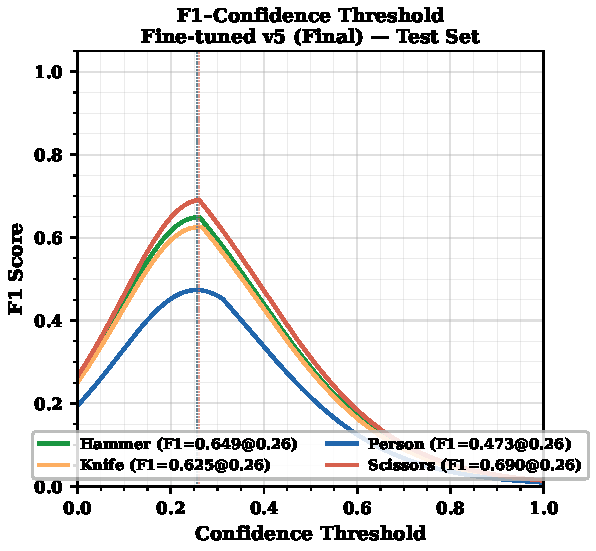
\includegraphics[width=\columnwidth]{fig10_f1_confidence.pdf}
\caption{Per-class F1 score versus confidence threshold.}
\label{fig:f1_conf}
\end{figure}


\subsection{Effect of Training Dataset Size}
Fine-tuned v1 (359 images) converges to a validation mAP of approximately 0.88, but its held-out test mAP is only 0.465, which is consistent with overfit to the Roboflow seed's narrow visual style under a single fixed split. The 0.414-point val-to-test drop motivated the v2 pass: v1 was not deployable as-is, and the gap indicated that additional distribution coverage from OpenImages was required. v2 (1{,}383 images) narrows the gap substantially (val 0.735, test 0.754), and v5 (4{,}982 images, 150 epochs) reaches val 0.817 and test 0.847. Within this corpus, dataset scale and diversity dominate; the methodological limits in Section~\ref{sec:dataset_limits} (targeted, not randomised, additions; single seed; same-corpus test split) prevent reading the trajectory as a scaling law for home-surveillance detectors at large. The progression is plotted in Fig.~\ref{fig:v1v2} and summarised in Table~\ref{tab:dataset_versions}.

\begin{figure}[ht!]
\centering
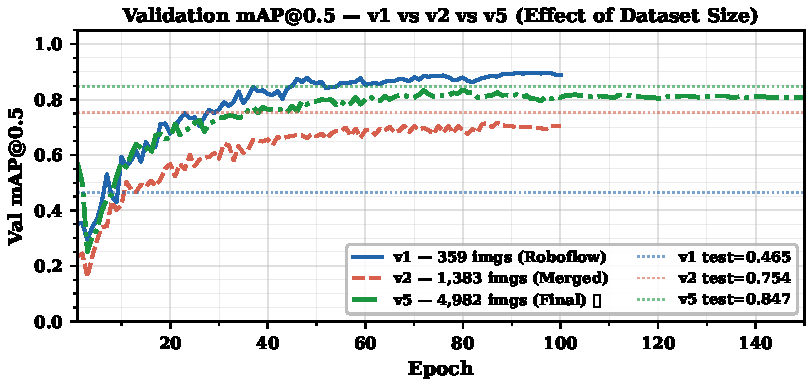
\includegraphics[width=\columnwidth]{fig11_v1_vs_v2_training.pdf}
\caption{Validation mAP{@}0.5 versus training-set size.}
\label{fig:v1v2}
\end{figure}

\begin{table}[ht!]
\caption{\textbf{Training Dataset Growth and Test mAP}}
\label{tab:dataset_versions}
\setlength{\tabcolsep}{2pt}
\centering\footnotesize
\begin{tabular}{|l|c|c|c|c|p{3.2cm}|}
\hline
\textbf{Ver.} & \textbf{Train} & \textbf{Total} & \textbf{Inst.} & \textbf{mAP50} & \textbf{Primary change} \\
\hline
v1 & 359   & 512   & $\sim$400    & 0.465 & Roboflow seed only \\
v2 & 1{,}383 & 1{,}730 & $\sim$1{,}300 & 0.754 & + OpenImages v7 (1{,}219 imgs) \\
v5 & 4{,}982 & 6{,}226 & 5{,}311       & 0.847 & + OI per-class (2{,}276 imgs) \\
\hline
\end{tabular}
\end{table}


\subsection{Validation-to-Test Generalisation Gap}
v1 shows a $\mathrm{val} - \mathrm{test} = 0.879 - 0.465 = 0.414$ mAP gap, characteristic of distribution overfit to the single-source seed. v2 closes the gap to $+0.019$ (test marginally above val), and v5 ends at $+0.030$ (test 0.847, val 0.817). A test score at or slightly above val on the expanded 4{,}982-image training set indicates the model does not collapse on the held-out split. The qualifier matters: the test split is drawn from the same author-curated corpus under the fixed seed of Section~\ref{sec:dataset_limits}, so this is a within-corpus result, not evidence of generalisation to an external benchmark. Fig.~\ref{fig:overfit} plots the progression.

\begin{figure}[!b]
\centering
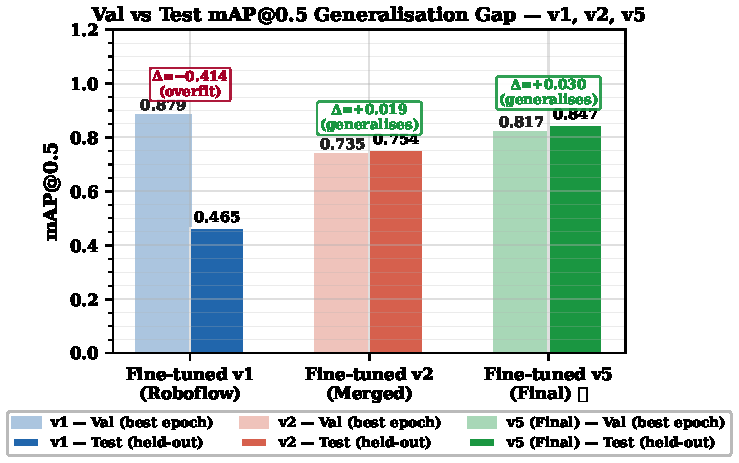
\includegraphics[width=\columnwidth]{fig12_overfitting_gap.pdf}
\caption{Validation-to-test mAP{@}0.5 gap across dataset versions.}
\label{fig:overfit}
\end{figure}


\subsection{Continuous-Deployment Telemetry and Functional Soak}
\label{sec:soak}
Two background services were left running on the deployed Pi~5 to give a first indication of how the full stack behaves outside a controlled bench test: a system-telemetry monitor that sampled host-level counters every 10~s for a 48-hour window, and a functional evaluation harness that drove the HTTP API of the Garuda web service on a 24-hour schedule. Neither campaign is a substitute for the multi-week in-situ study of Section~\ref{sec:conclusion}, but they bound short-horizon stability on the deployed hardware.

\paragraph*{48-hour system telemetry}
The monitor recorded CPU utilisation (overall and per-core), RAM, SoC temperature, network throughput, load average, disk occupancy, throttle flag, and the liveness of the Garuda web service over a 48-hour scheduled window. Of the $N_{\text{ideal}} = 48 \times 3600 / 10 = 17{,}280$ expected 10~s samples, the logger retained $N = 13{,}540$, covering $N \cdot 10 / 3600 \approx 37.6$~h (about 78\% of the nominal window). The shortfall arose from a service restart and an \texttt{rsyslog} rotation that interrupted the sampler; it biases the coverage of the time-axis but does not distort the per-sample aggregates reported below. Across that window the CPU ran at mean $34.7\%$ / median $48.2\%$ / p95 $66.2\%$, RAM at mean $18.0\%$ (2{,}710~MB of 16~GB) / p95 $24.9\%$ (3{,}803~MB), and SoC temperature at mean $65.5\,^\circ$C / median $72.2\,^\circ$C / p95 $77.1\,^\circ$C / max $84.8\,^\circ$C. The mean-below-median ordering on CPU and SoC reflects a bimodal occupancy distribution: two sampler-startup cool-down transients and a brief post-restart idle stretch contribute a left tail of low-load and low-temperature samples that drags the mean down without moving the median, which tracks the sustained operating regime. The 1-minute load average held a median of $2.99$ against four physical cores. Disk occupancy did not drift outside $8.2$--$8.3\%$, so the log-rotation path of Section~\ref{sec:cpu_services} absorbed the full campaign without spill-over. The sticky \texttt{vcgencmd get\_throttled} bit was observed to latch during the run, consistent with peak SoC temperatures in the low-$80\,^\circ$C range; no sample reported under-voltage. The sticky flag is not read as evidence of sustained frequency capping, but is surfaced here as a thermal-headroom reminder rather than hidden. Fig.~\ref{fig:telemetry48h} plots CPU, RAM, and SoC temperature against elapsed time.

\begin{figure}[ht!]
\centering

\includegraphics[width=\columnwidth]{fig14_48h_telemetry.pdf}
\caption{48~h continuous host-level telemetry on the deployed Pi~5.}\label{fig:telemetry48h}
\end{figure}

\paragraph*{24-hour functional evaluation}
In parallel, a harness exercised every CPU-side engine (presence monitor, snapshot, email, chat, clip recorder, and the heartbeat of the deadman watchdog) through the authenticated HTTP API, tailed the permanent detection, system, and voice logs, and wrote per-probe and per-event records over a 24-hour window (intermediate restarts contributed a sub-two-hour wall-clock gap that is negligible at this duration). The harness queried the deadman heartbeat endpoint at an effective cadence of $t_h \approx 22\,\mathrm{h} \cdot 3600 / 3{,}351 \approx 23.6$~s (host-scheduled, drifting against the 10~s deadman-internal loop of Table~\ref{tab:operational_params}); the endpoint responded successfully on $3{,}332$ of $3{,}351$ probes ($99.43\%$), the chat API answered with a mean round-trip latency of $0.526$~s over the 10 probes that returned a 200 response (of 13 attempted), and the detection log accumulated 521 watch-level events with 0 danger-level events and 0 spurious email alerts, giving no false critical-alarm escalations during the soak. Engines dependent on external services showed the expected partial failures that an offline-tolerant build should surface: $4/7$ email probes, $10/13$ chat probes, $11/13$ snapshot probes, and $19/21$ presence probes succeeded. The voice-assistant log recorded \texttt{"No Default Input Device Available"} throughout, because the campaign ran headless without a microphone attached; this is a configuration artefact, not a Narada defect, and it is the reason Section~\ref{sec:conclusion} still lists on-device TTS and end-to-end voice validation as follow-up work. These 24- and 48-hour numbers are not promoted to a multi-week stability claim; they are reported as what they are: short-horizon evidence that the deployed stack does not leak memory, does not thermally run away, and does not emit false danger alerts over a 24- / 48-hour window on the target hardware.


\section{Conclusion}
\label{sec:conclusion}
This paper presents a privacy-first edge-AI home-security platform in which every frame of inference stays on the device. A Raspberry~Pi~5 (16~GB, 2.8~GHz, with active cooler) paired with a Hailo-8L AI HAT+ hosts the full inference stack (a fine-tuned YOLOv8s detector, a MobileNetV2 Safe/Weapon verifier, and a MiDaS Small depth-variance pre-filter) at 52.2~FPS and 18.4~ms on-chip latency, leaving the CPU free for the FastAPI web server, the Narada voice assistant, presence monitoring, the deadman watchdog, and the logging engine. The 52.2~FPS envelope stays flat across every operating mode, and that flatness is a property of the asynchronous, CPU-pinned, bounded-queue pipeline rather than of any single model.

On the model side, the v1$\rightarrow$v5 progression yields a test-mAP delta of $\Delta_{15} = 0.847 - 0.465 = 0.382$ with a validation-to-test gap of $+0.030$ at v5, so dataset scale and diversity dominate the contribution rather than architectural changes. Writing $\sigma_{\text{run}} \approx 0.02$ for the typical YOLO fine-tune run-to-run mAP variance at this scale, the signal-to-noise ratio of the jump is $\Delta_{15} / \sigma_{\text{run}} \approx 19$, large enough to reject chance, though the result is interpreted as an existence proof of within-corpus scaling rather than a generalisable law, given single-seed, single-split, and targeted-addition qualifications. The INT8 HEF re-evaluated on-chip over the same 622-image test split reaches mAP{@}0.5 = 0.854 ($\Delta = +0.007$ vs.\ FP32) and mAP{@}0.5:0.95 = 0.682 ($\Delta = +0.012$); quantisation contributes no measurable accuracy loss. The 22.9~MB artefact sustains 52.2~FPS at $5.89 \pm 1.43$~W of measured board power under concurrent inference and service load, with a $+3.8^\circ$C NPU surface-temperature rise.

Against cloud cameras, an illustrative three-year total-cost-of-ownership sketch (Ring~Stick~Up~Cam US\$79.99~\cite{b33} + Ring~AI~Pro US\$199.99/yr~\cite{b34}; Google~Nest~Cam US\$179.99~\cite{b35} + Home~Premium US\$100--200/yr~\cite{b36}; SimpliSafe US\$149.99~\cite{b37} + self-monitoring US\$120/yr~\cite{b38}; all prices accessed April~2026) places the subscription-backed comparators at US\$680--910, while the proposed system incurs its one-time US\$411 BOM (Table~\ref{tab:bom}) plus a three-year electricity cost of $5.89\,\mathrm{W} \cdot 3\,\mathrm{yr} \cdot 8{,}760\,\mathrm{h/yr} \cdot 0.15\,\$\mathrm{/kWh} / 1000 \approx \$23$ at US residential tariffs, which is the only recurring line item. Premium local-first comparators (eufyCam~S3~Pro~\cite{b39}, Reolink~Argus~4~Pro~\cite{b40}) avoid the subscription but trade it for higher upfront price and narrower platform scope. Three caveats bound this comparison and it should be read as illustrative rather than as a controlled price study: (a) the proposed system's BOM is priced on the Indian market in INR and converted at a single point-in-time rate ($1\,\text{USD}=92.6\,\text{INR}$, Table~\ref{tab:bom}), whereas the commercial comparators are US list prices, so the two currencies and two retail markets are not matched; (b) list prices fluctuate, promotions and tax are excluded, and the subscription tiers used here are mid-band rather than cheapest-available; (c) the commercial units are single-camera appliances and the proposed system is a multi-service platform, so the comparison is platform-functional-scope parity rather than per-camera parity. The claim is cost-effectiveness on total-cost-of-ownership at this platform scope, not on single-camera day-one sticker price, and the paper does not claim to replace any specific commercial product without the continuous-deployment evaluation flagged below.

Three future-work directions tighten the result into a deployment claim: (i) an in-situ security evaluation covering alert precision/recall on unstaged multi-day video, nuisance-condition sweeps, physical replay-attack testing, fault injection on the tunnel and alert paths, a multi-week stability study, and a matched-stimulus commercial-camera comparison; (ii) a generalisability re-analysis of the dataset trajectory with a repeated-seed/repeated-split v1$\rightarrow$v5 sweep, an inter-annotator-agreement study, an external benchmark, and an open-set verifier evaluation with household-clutter negatives; and (iii) scoped component upgrades, namely a proper face anti-spoof stage on in-domain data, a broader class vocabulary, a temporal activity-recognition layer, and on-device TTS for Narada.



\appendices
\section{Hardware, Software, and Model Specifications}
\label{sec:specs}
This appendix consolidates the hardware, software, and model specifications of the deployed system so that the results reported in Section~\ref{sec:results} can be reproduced on comparable equipment. Only the deployed configuration is listed; development-time alternatives are not included.

\subsection{Hardware}
Table~\ref{tab:hw_specs} lists the host board, accelerator, camera, storage, and network interface used for every reported measurement.

\begin{table}[ht!]
\caption{\textbf{Hardware Specification}}
\label{tab:hw_specs}
\setlength{\tabcolsep}{3pt}
\centering\footnotesize
\begin{tabular}{|l|p{4.0cm}|}
\hline
\textbf{Component} & \textbf{Specification} \\
\hline
Host board & Raspberry Pi~5 (BCM2712) \\
CPU & Quad-core Arm Cortex-A76 \\
CPU clock (overclocked) & 2.8~GHz (\texttt{arm\_freq=2800}) \\
RAM & 16~GB LPDDR4X-4267 \\
Storage & 1~TB Crucial SATA SSD (USB~3.0 enclosure) \\
Neural accelerator & Hailo-8L AI HAT+ (13~TOPS, INT8) \\
NPU interface & PCIe Gen3~$\times$1 (M.2 M-key) \\
Device node & \texttt{/dev/hailo0} \\
Camera & Raspberry Pi Camera Module~v3 (Sony IMX708) \\
Camera interface & CSI-2 MIPI (libcamera) \\
Networking & 802.11ac Wi-Fi \\
Power supply & 5~V / 5~A USB-C (official PSU) \\
Estimated BOM (Table~\ref{tab:bom}) & US\$411 \\
\hline
\end{tabular}
\end{table}

\begin{table}[ht!]
\caption{\textbf{Itemised Bill of Materials (2026 list prices; INR at point of sale, USD at $1\,\text{USD}=92.6\,\text{INR}$)}}
\label{tab:bom}
\setlength{\tabcolsep}{3pt}
\centering\footnotesize
\begin{tabular}{|l|r|r|}
\hline
\textbf{Component} & \textbf{INR} & \textbf{USD} \\
\hline
Raspberry Pi~5 (8~GB)\textsuperscript{a} \emph{(robu.in SKU~1749034)}          & 19{,}618 & 211.86 \\
Hailo-8L AI HAT+ (13~TOPS)  \emph{(SKU~R182940)}                                &  7{,}469 &  80.66 \\
Raspberry Pi Camera Module~v3 \emph{(SKU~1441079)}                              &  3{,}099 &  33.47 \\
Consistent 512~GB 2.5" SATA SSD \emph{(amazon.in)}                               &  5{,}899 &  63.70 \\
Official Raspberry Pi~5 27~W USB-C PSU \emph{(amazon.in)}                       &  1{,}512 &  16.33 \\
Official Raspberry Pi~5 Active Cooler \emph{(SKU~1749017)}                      &     488 &   5.27 \\
\hline
\textbf{Total BOM}                                                              & \textbf{38{,}085} & \textbf{411.28} \\
\hline
\end{tabular}\\[2pt]
\raggedright\scriptsize Prices reflect list values at the time of procurement (robu.in / amazon.in, India) and exclude tax, shipping, and consumables. Electricity is a separate operating cost (see Section~\ref{sec:conclusion}).\\
\textsuperscript{a}The deployed unit used for every reported measurement carries 16~GB; the 8~GB variant is priced here because the 48~h telemetry in Section~\ref{sec:soak} shows a p95 of 24.9\% of 16~GB (3.8~GB), so 8~GB reproduces the workload with headroom at lower cost.
\end{table}

\subsection{Software Stack}
The software stack is summarised in Table~\ref{tab:sw_specs}. The Hailo driver is installed as a DKMS module so that kernel upgrades do not break the PCIe interface, and all Python services run under a single virtual environment activated by the \texttt{setup\_env.sh} script shipped with the project.

\begin{table}[ht!]
\caption{\textbf{Software Stack Specification}}
\label{tab:sw_specs}
\setlength{\tabcolsep}{3pt}
\centering\footnotesize
\begin{tabular}{|l|p{4.3cm}|}
\hline
\textbf{Layer} & \textbf{Version / Package} \\
\hline
Operating system & Raspberry Pi OS (64-bit, Debian 12) \\
Kernel & Linux 6.12.x \\
Hailo driver & \texttt{hailo\_pci} 4.20.0 (DKMS) \\
Hailo runtime & HailoRT 4.20.0 \\
Hailo compiler & Hailo Dataflow Compiler v3.33.1 \\
TAPPAS framework & 3.28.x / 3.31.0 \\
GStreamer & 1.22 \\
Python & 3.11 \\
Web framework & FastAPI + Uvicorn \\
ASGI media & aiortc (WebRTC), \texttt{python-multipart} \\
Speech & \texttt{SpeechRecognition}, \texttt{PyAudio} \\
LLM backend & Groq API, \texttt{gpt-oss-120b} (free tier) \\
Auth primitives & \texttt{hashlib.pbkdf2\_hmac}, \texttt{secrets} \\
Crypto & AES-256-GCM (\texttt{cryptography}) \\
Remote exfiltration & \texttt{paramiko} (SSH) \\
Event database & SQLite 3.40 \\
Public ingress & Cloudflare Tunnel (\texttt{cloudflared}) \\
\hline
\end{tabular}
\end{table}

\subsection{Models}
Three neural networks are deployed, all compiled to INT8 HEF files for the Hailo-8L. The primary detector is a YOLOv8s model fine-tuned on the four-class dataset (Section~\ref{sec:dataset}), trained for 150 epochs, and quantised with the Hailo DFC v3.33.1. The classifier is a MobileNetV2 that labels person crops as Safe or Weapon. The third is MiDaS Small, used only as a coarse depth-variance pre-filter (not a face anti-spoof decision; Section~\ref{sec:antispoof_eval}). Table~\ref{tab:model_specs} lists all deployed artefacts.

\begin{table}[ht!]
\caption{\textbf{Deployed Models and Artefacts (Hailo-8L)}}
\label{tab:model_specs}
\setlength{\tabcolsep}{2pt}
\centering\footnotesize
\resizebox{\columnwidth}{!}{%
\begin{tabular}{|l|c|l|c|c|}
\hline
\textbf{Artefact} & \textbf{Size} & \textbf{Task} & \textbf{FPS} & \textbf{Latency} \\
\hline
\texttt{best\_v5.hef} (YOLOv8s)          & 22.9~MB & 4-class detection   & 52.2 & 18.4~ms \\
\texttt{mobilenetv2\_garuda.hef}          & 7.1~MB  & Safe/Weapon crop cls. & 500+  & $<$2~ms \\
\texttt{midas\_depth.hef} (MiDaS Small)  & 35~MB   & Monocular depth     & 200+  & $<$5~ms \\
\texttt{libyolo\_hailortpp\_post.so}      & 561~KB  & Custom-label NMS    & ---   & --- \\
\hline
\end{tabular}%
}
\end{table}


\subsection{Service-side Parameters}
\label{sec:service_params}
The per-engine implementation parameters referenced from Section~\ref{sec:cpu_services} are split into two tables for readability: the security-relevant primitives (Table~\ref{tab:security_params}) and the operational/scheduling values (Table~\ref{tab:operational_params}). None of these values is load-bearing for any reported result; they are listed only for reproducibility.

\begin{table}[ht!]
\caption{\textbf{Security-relevant Primitives}}
\label{tab:security_params}
\setlength{\tabcolsep}{3pt}
\centering\footnotesize
\begin{tabular}{|l|p{4.0cm}|}
\hline
\textbf{Parameter} & \textbf{Value} \\
\hline
PBKDF2 iterations & 600{,}000 (SHA-256, per-user salt) \\
Session token & HTTP-only cookie, server-side lookup \\
Admin 2FA & 6-digit OTP via SMTPS, 10-min expiry \\
Evidence-clip cipher & AES-256-GCM, key from env var \\
Evidence-clip transport & SSH (\texttt{paramiko}) \\
Privacy-mode blur kernel & Gaussian, $k{=}51$~px, $\sigma{=}30$~px \\
Public ingress & Cloudflare Tunnel \\
\hline
\end{tabular}
\end{table}

\begin{table}[ht!]
\caption{\textbf{Operational and Scheduling Parameters}}
\label{tab:operational_params}
\setlength{\tabcolsep}{3pt}
\centering\footnotesize
\begin{tabular}{|l|p{4.0cm}|}
\hline
\textbf{Parameter} & \textbf{Value} \\
\hline
Alert SMTPS cooldown (per label) & 60~s \\
Mode-flag set & DND, email-off, idle, emergency, privacy \\
Schedule-monitor poll & 30~s \\
ARP presence poll & 30~s \\
Presence grace window & 90~s \\
Deadman heartbeat check & 10~s \\
Deadman silence threshold & 180~s \\
FastAPI bind & \texttt{localhost:8080} (Uvicorn) \\
REST routes (approx.) & 45 \\
Live-video channels & MJPEG, WebSocket binary, WebRTC (aiortc) \\
Log rotation & size-based (10~MB, single rollover), append-only \\
Catch-up endpoint & \texttt{/api/events?since=T} (SQLite-backed) \\
\hline
\end{tabular}
\end{table}


\subsection{v6 Fine-tune: Full Configuration and Per-Class Regression Analysis}
\label{sec:v6_details}
The compressed v6 discussion in Section~\ref{sec:person_recall_discussion} is expanded here for reproducibility. The v6 fine-tune used a fresh YOLOv8s initialisation trained on an expanded corpus of 4{,}720 primary-class Person images (13{,}014 Person instances), with an additional 1{,}903 Open Images Person photographs drawn under a different seed to raise crowded-scene diversity. The augmentation schedule was pushed beyond the v5 defaults to \texttt{copy\_paste}$=0.5$, \texttt{mixup}$=0.2$, and \texttt{label\_smoothing}$=0.05$, with 200 training epochs and a later mosaic-close schedule tuned for crowded scenes.

The per-class outcome at the deployed confidence threshold was: overall test mAP{@}0.5 $0.847 \to 0.741$; Person recall $0.609 \to 0.481$; Hammer recall $0.848 \to 0.765$; Knife recall $0.817 \to 0.913$ (the only class to improve); Scissors recall held near 0.921. Lowering the confidence threshold to 0.10 recovered overall mAP only to 0.766 and did not move Person recall, which rules out a pure threshold-tuning explanation.

The v6 run changed two things at once relative to v5 (a larger and differently-composed Person subset, and a stronger augmentation schedule with \texttt{copy\_paste}, \texttt{mixup}, and \texttt{label\_smoothing} all enabled), so the regression cannot be attributed to either factor individually without a controlled A/B. A corpus-only v6a (v6 corpus, v5 augmentation) and an augmentation-only v6b (v5 corpus, v6 augmentation) sweep are flagged as future work alongside the other dataset-trajectory re-analyses in Section~\ref{sec:conclusion}. What the v6 run does establish is a directional signal: a one-shot re-balancing toward the rarest failure class, with the augmentation stack pushed beyond the defaults, did not improve the test envelope; v5 was therefore retained as the Pareto-optimal operating point on this test split because it keeps the alert-class recalls (Hammer 0.848, Knife 0.817, Scissors 0.929) intact while the v6 run gave up Hammer and overall mAP in exchange for the single Knife-recall gain. The v6 experiment is reported as a documented negative result that motivates the four architectural directions flagged in the main text, not as a causal explanation of what broke.




\section*{Code and Data Availability}
\label{sec:code_data}
The complete codebase for the work reported here (Hailo GStreamer pipeline, FastAPI web server, voice assistant, authentication and evidence-capture subsystems, dataset-preparation scripts, and the evaluation artefacts referenced in Section~\ref{sec:results}, comprising INT8 mAP, open-set verifier test, power-measurement traces, and the 720~s FPS time-series used to produce Fig.~\ref{fig:fps_ts}) is released under an MIT license at \url{https://github.com/Manikanta25055/Garuda_26}. The deployed HEF artefacts (\texttt{best\_v5.hef} for the primary detector, \texttt{mobilenetv2\_garuda.hef} for the secondary verifier, and \texttt{midas\_depth.hef} for the depth-variance pre-filter) and the \texttt{libyolo\_hailortpp\_post.so} post-processing library are included in the same repository. The dataset split itself is not redistributed directly, but the SHA-256 manifest of image identifiers and the per-split label files are available alongside the code so that an equivalent split can be reconstructed from the upstream Roboflow Universe and OpenImages v7 sources (both CC BY 4.0) using the scripts in the repository.

\section*{Ethics and Data-Use Statement}
\label{sec:ethics}
No human-subjects study, no interaction with identifiable individuals, and no collection of original video or biometric data from third parties was undertaken for this work, and accordingly no Institutional Review Board (IRB) or ethics-committee approval was required. All training and evaluation imagery for the four-class detector was drawn from publicly released, permissively licensed corpora (Roboflow Universe ``Knives \& Scissors Training v2'' and Open Images v7, both CC BY 4.0); the upstream providers are responsible for consent and rights clearance on those images, and no identities are inferred or reported in this paper. The CelebA-Spoof subset used for the short sanity check of Section~\ref{sec:antispoof_eval} was accessed from the authors' publicly released research distribution for academic, non-commercial research use only. IEEE Access publication is compatible with these terms because this paper is a non-commercial academic research output and the dataset is not redistributed, republished, or otherwise made available through this paper or through the associated code repository. Specifically: (i) no CelebA-Spoof image, crop, thumbnail, or rendered example appears in any figure or table of this paper; (ii) only a single aggregate scalar (AUC $= 0.563$ with a $95\%$ confidence interval over a 600-image subset) and the derived $z$-score are reported, and no per-image, per-subject, per-identity, per-demographic, or per-attribute statistic is released; (iii) no identity, demographic, or attribute inference is performed and no model weights or features derived from CelebA-Spoof are released; (iv) the evaluation code in the associated repository loads images from a user-supplied local copy of the dataset and neither bundles nor redistributes the data itself. The subset is used solely to bound the scope of the depth-variance pre-filter, and is cited as a reference-only evaluation artefact. All operational imagery captured on the deployed Raspberry Pi Camera during development was recorded in the first author's private residence with the consent of the household; no such footage is redistributed with this paper. Evidence clips produced by the deployed system are encrypted at rest (AES-256-GCM) and remain on the user's own hardware; the system is designed so that raw video never leaves the device to a third-party service. Commercial product names and prices cited in Section~\ref{sec:conclusion} are used for the sole purpose of cost-of-ownership comparison and do not constitute an endorsement.

\begin{thebibliography}{00}

\bibitem{b2} J.~Redmon, S.~Divvala, R.~Girshick, and A.~Farhadi, ``You only look once: Unified, real-time object detection,'' in \emph{Proc. IEEE Conf. Comput. Vis. Pattern Recognit. (CVPR)}, Las Vegas, NV, USA, 2016, pp.~779--788.

\bibitem{b1} Z.~Xu, J.~Li, and M.~Zhang, ``A surveillance video real-time analysis system based on edge-cloud and FL-YOLO cooperation in coal mine,'' \emph{IEEE Access}, vol.~9, pp.~161~498--161~512, 2021.

\bibitem{b5} R.~Al~Amin, M.~Hasan, V.~Wiese, and R.~Obermaisser, ``FPGA-based real-time object detection and classification system using YOLO for edge computing,'' \emph{IEEE Access}, vol.~12, pp.~61~080--61~093, 2024.

\bibitem{b6} C.~Dong, C.~Pang, Z.~Li, X.~Zeng, and X.~Hu, ``PG-YOLO: A novel lightweight object detection method for edge devices in industrial Internet of Things,'' \emph{IEEE Access}, vol.~10, pp.~40~177--40~186, 2022.

\bibitem{b25} H.~Alqahtani, M.~A.~Cheema, and A.~N.~Toosi, ``Benchmarking deep learning models for object detection on edge computing devices,'' arXiv preprint arXiv:2409.16808, Sep.~2024. [Preprint, not peer reviewed.]

\bibitem{b26} D.~Rey, A.~M.~Bernardos, P.~Dobrzycki, A.~Carrami\~{n}ana, L.~Bergesio, J.~A.~Besada, and J.~R.~Casar, ``A performance analysis of YOLOv8 on edge devices for aerial imagery,'' arXiv preprint arXiv:2502.15737, Feb.~2025. [Preprint, not peer reviewed.]

\bibitem{b27} W.~Ullah, T.~Hussain, F.~U.~M.~Ullah, M.~Y.~Lee, and S.~W.~Baik, ``TransCNN: Hybrid CNN and transformer mechanism for surveillance anomaly detection,'' \emph{Eng. Appl. Artif. Intell.}, vol.~123, Part~B, Art.~no.~106173, Aug.~2023, doi: 10.1016/j.engappai.2023.106173.

\bibitem{b29} M.~B.~Musthafa, S.~Huda, T.~T.~Nguyen, Y.~Kodera, and Y.~Nogami, ``Optimized ensemble deep learning for real-time intrusion detection on resource-constrained Raspberry Pi devices,'' \emph{IEEE Access}, vol.~13, pp.~113~544--113~556, 2025, doi: 10.1109/ACCESS.2025.3584373.

\bibitem{b9} G.~Jocher, A.~Chaurasia, and J.~Qiu, ``Ultralytics YOLOv8,'' 2023. [Online]. Available: https://github.com/ultralytics/ultralytics [Accessed: Apr.~19, 2026].

\bibitem{b10} Hailo Technologies Ltd., ``TAPPAS --- Hailo's AI application development framework,'' 2024. [Online]. Available: https://github.com/hailo-ai/tappas [Accessed: Apr.~19, 2026].

\bibitem{b13} GStreamer Team, ``GStreamer: Open source multimedia framework,'' 2024. [Online]. Available: https://gstreamer.freedesktop.org [Accessed: Apr.~19, 2026].

\bibitem{b11} Raspberry Pi Ltd., ``Raspberry Pi 5 product brief,'' 2023. [Online]. Available: https://www.raspberrypi.com/products/raspberry-pi-5/ [Accessed: Apr.~19, 2026].

\bibitem{b4} G.~Bueno \emph{et~al.}, ``Real-time edge computing vs.\ GPU-accelerated pipelines for low-cost microscopy applications,'' \emph{Electronics}, vol.~14, no.~6, Art.~no.~930, 2025.

\bibitem{b18} M.~T.~Bhatti, M.~G.~Khan, M.~Aslam, and M.~J.~Fiaz, ``Weapon detection in real-time CCTV videos using deep learning,'' \emph{IEEE Access}, vol.~9, pp.~34~366--34~382, 2021, doi: 10.1109/ACCESS.2021.3059170.

\bibitem{b30} L.~Sumi and S.~Dey, ``YOLOv5-based weapon detection systems with data augmentation,'' \emph{Int. J. Computers and Applications} (Taylor \& Francis), vol.~45, no.~4, pp.~288--296, 2023, doi: 10.1080/1206212X.2023.2182966.

\bibitem{b19} A.~Yadav, N.~Gupta, and A.~Sharma, ``YOLOv7-DarkVision: Weapon detection in low-light surveillance videos with illumination-aware enhancement,'' \emph{Digital Signal Processing}, vol.~145, Art.~no.~104342, 2024, doi: 10.1016/j.dsp.2023.104342.

\bibitem{b20} A.~Amado-Garf\'{i}as, J.~F.~Mart\'{i}nez-Trinidad, J.~A.~Carrasco-Ochoa, and J.~C.~Ram\'{i}rez-Cruz, ``Enhancing armed-person detection in surveillance by combining YOLOv4, geometric heuristics, and classical machine-learning verifiers,'' \emph{IEEE Access}, vol.~12, pp.~116~732--116~746, 2024, doi: 10.1109/ACCESS.2024.3442728.

\bibitem{b32} N.~Hnoohom, P.~Chotivatunyu, and A.~Jitpattanakul, ``ACF: An armed CCTV footage dataset for enhancing weapon detection,'' \emph{Sensors (MDPI)}, vol.~22, no.~19, Art.~no.~7158, 2022, doi: 10.3390/s22197158.

\bibitem{b28} E.~I.~R.~Jacob \emph{et~al.}, ``An enhanced surveillance system for gun and knife detection using YOLOv8 and Raspberry Pi,'' in \emph{Proc. IEEE Int. Conf. Communication, Computing and Internet of Things (IC3IoT)}, Chennai, India, 2024, pp.~1--6, doi: 10.1109/IC3IoT60841.2024.10550256.

\bibitem{b21} Z.~Yu, Y.~Qin, X.~Li, C.~Zhao, Z.~Lei, and G.~Zhao, ``Deep learning for face anti-spoofing: A survey,'' \emph{IEEE Trans. Pattern Anal. Mach. Intell.}, vol.~45, no.~5, pp.~5609--5631, May 2023, doi: 10.1109/TPAMI.2022.3215850.

\bibitem{b22} Y.~Zhang, Z.~Yin, Y.~Li, G.~Yin, J.~Yan, J.~Shao, and Z.~Liu, ``CelebA-Spoof: Large-scale face anti-spoofing dataset with rich annotations,'' in \emph{Proc. Eur. Conf. Comput. Vis. (ECCV)}, Glasgow, UK, 2020, pp.~70--85.

\bibitem{b23} Q.~Zhou, K.~Y.~Zhang, T.~Yao, X.~Lu, S.~Ding, and L.~Ma, ``Test-time domain generalization for face anti-spoofing,'' in \emph{Proc. IEEE/CVF Conf. Comput. Vis. Pattern Recognit. (CVPR)}, Seattle, WA, USA, 2024, pp.~175--185.

\bibitem{b14} R.~Ranftl, K.~Lasinger, D.~Hafner, K.~Schindler, and V.~Koltun, ``Towards robust monocular depth estimation: Mixing datasets for zero-shot cross-dataset transfer,'' \emph{IEEE Trans. Pattern Anal. Mach. Intell.}, vol.~44, no.~3, pp.~1623--1637, Mar. 2022.

\bibitem{b15} M.~Sandler, A.~Howard, M.~Zhu, A.~Zhmoginov, and L.-C.~Chen, ``MobileNetV2: Inverted residuals and linear bottlenecks,'' in \emph{Proc. IEEE Conf. Comput. Vis. Pattern Recognit. (CVPR)}, Salt Lake City, UT, USA, 2018, pp.~4510--4520.

\bibitem{b31} O.~Taiwo, A.~E.~Ezugwu, O.~N.~Oyelade, and M.~S.~Almutairi, ``Enhanced intelligent smart home control and security system based on deep learning model,'' \emph{Wireless Commun. Mobile Comput.} (Wiley/Hindawi), vol.~2022, Art.~no.~9307961, 2022, doi: 10.1155/2022/9307961.

\bibitem{b24} B.~Blackshear, ``Frigate --- NVR with realtime local object detection for IP cameras,'' 2024. [Online]. Available: https://github.com/blakeblackshear/frigate [Accessed: Apr.~19, 2026].

\bibitem{b12} S.~Ram\'{i}rez, ``FastAPI --- Modern, fast web framework for building APIs with Python,'' 2019. [Online]. Available: https://fastapi.tiangolo.com [Accessed: Apr.~19, 2026].

\bibitem{b17} Cloudflare, Inc., ``Cloudflare Tunnel documentation,'' 2024. [Online]. Available: https://developers.cloudflare.com/cloudflare-one/connections/connect-networks/ [Accessed: Apr.~19, 2026].

\bibitem{b16} B.~Kaliski, ``PKCS \#5: Password-based cryptography specification version 2.0,'' RFC 2898, Internet Eng. Task Force, Sep. 2000.

\bibitem{b41} OWASP Foundation, ``Password Storage Cheat Sheet,'' OWASP Cheat Sheet Series, 2024. [Online]. Available: \url{https://cheatsheetseries.owasp.org/cheatsheets/Password_Storage_Cheat_Sheet.html} [Accessed: Apr.~19, 2026].

\bibitem{b3} Hailo Technologies Ltd., ``Hailo-8L M.2 AI acceleration module product brief,'' 2024. [Online]. Available: https://hailo.ai/products/ai-accelerators/hailo-8l-ai-accel-for-ai-light-applications/ [Accessed: Apr.~19, 2026].

\bibitem{b33} Ring LLC, ``Stick Up Cam Battery,'' product page, 2026. [Online]. Available: https://ring.com/products/stick-up-cam-battery [Accessed: Apr.~19, 2026].

\bibitem{b34} Ring LLC, ``Ring Protect plans,'' 2026. [Online]. Available: https://ring.com/protect-plans [Accessed: Apr.~19, 2026].

\bibitem{b35} Google LLC, ``Nest Cam (battery),'' Google Store product page, 2026. [Online]. Available: https://store.google.com/us/product/nest\_cam\_battery [Accessed: Apr.~19, 2026].

\bibitem{b36} Google LLC, ``Google Home Premium (formerly Nest Aware),'' Google Store, 2026. [Online]. Available: https://store.google.com/us/product/nest\_aware [Accessed: Apr.~19, 2026].

\bibitem{b37} SimpliSafe, Inc., ``Outdoor Security Camera Bundle,'' product page, 2026. [Online]. Available: https://simplisafe.com/outdoor-security-camera-bundle [Accessed: Apr.~19, 2026].

\bibitem{b38} SimpliSafe, Inc., ``Monitoring plans,'' support page, 2026. [Online]. Available: https://support.simplisafe.com/page/monitoring-plans [Accessed: Apr.~19, 2026].

\bibitem{b39} Anker Innovations Ltd., ``eufyCam S3 Pro 2-Cam Kit,'' eufy product page, 2026. [Online]. Available: https://www.eufy.com/products/t88921w1 [Accessed: Apr.~19, 2026].

\bibitem{b40} Reolink Digital Technology Co., Ltd., ``Argus 4 Pro,'' product page, 2026. [Online]. Available: https://reolink.com/us/product/argus-4-pro/ [Accessed: Apr.~19, 2026].

\end{thebibliography}

\raggedbottom
% Pack biographies tight: kill the stretchy vskip and the force-next-column check
% that the IEEEbiography macro inserts before each entry.
\makeatletter
\patchcmd{\IEEEbiography}{\vskip \@IEEEBIOskipN plus 1fil minus 0\baselineskip}{\vskip \@IEEEBIOskipN}{}{}
\patchcmd{\IEEEbiography}{\@IEEEtranneedspace{\@IEEEtrantmpdimenA}{\relax}}{}{}{}
\makeatother

\begin{IEEEbiography}[{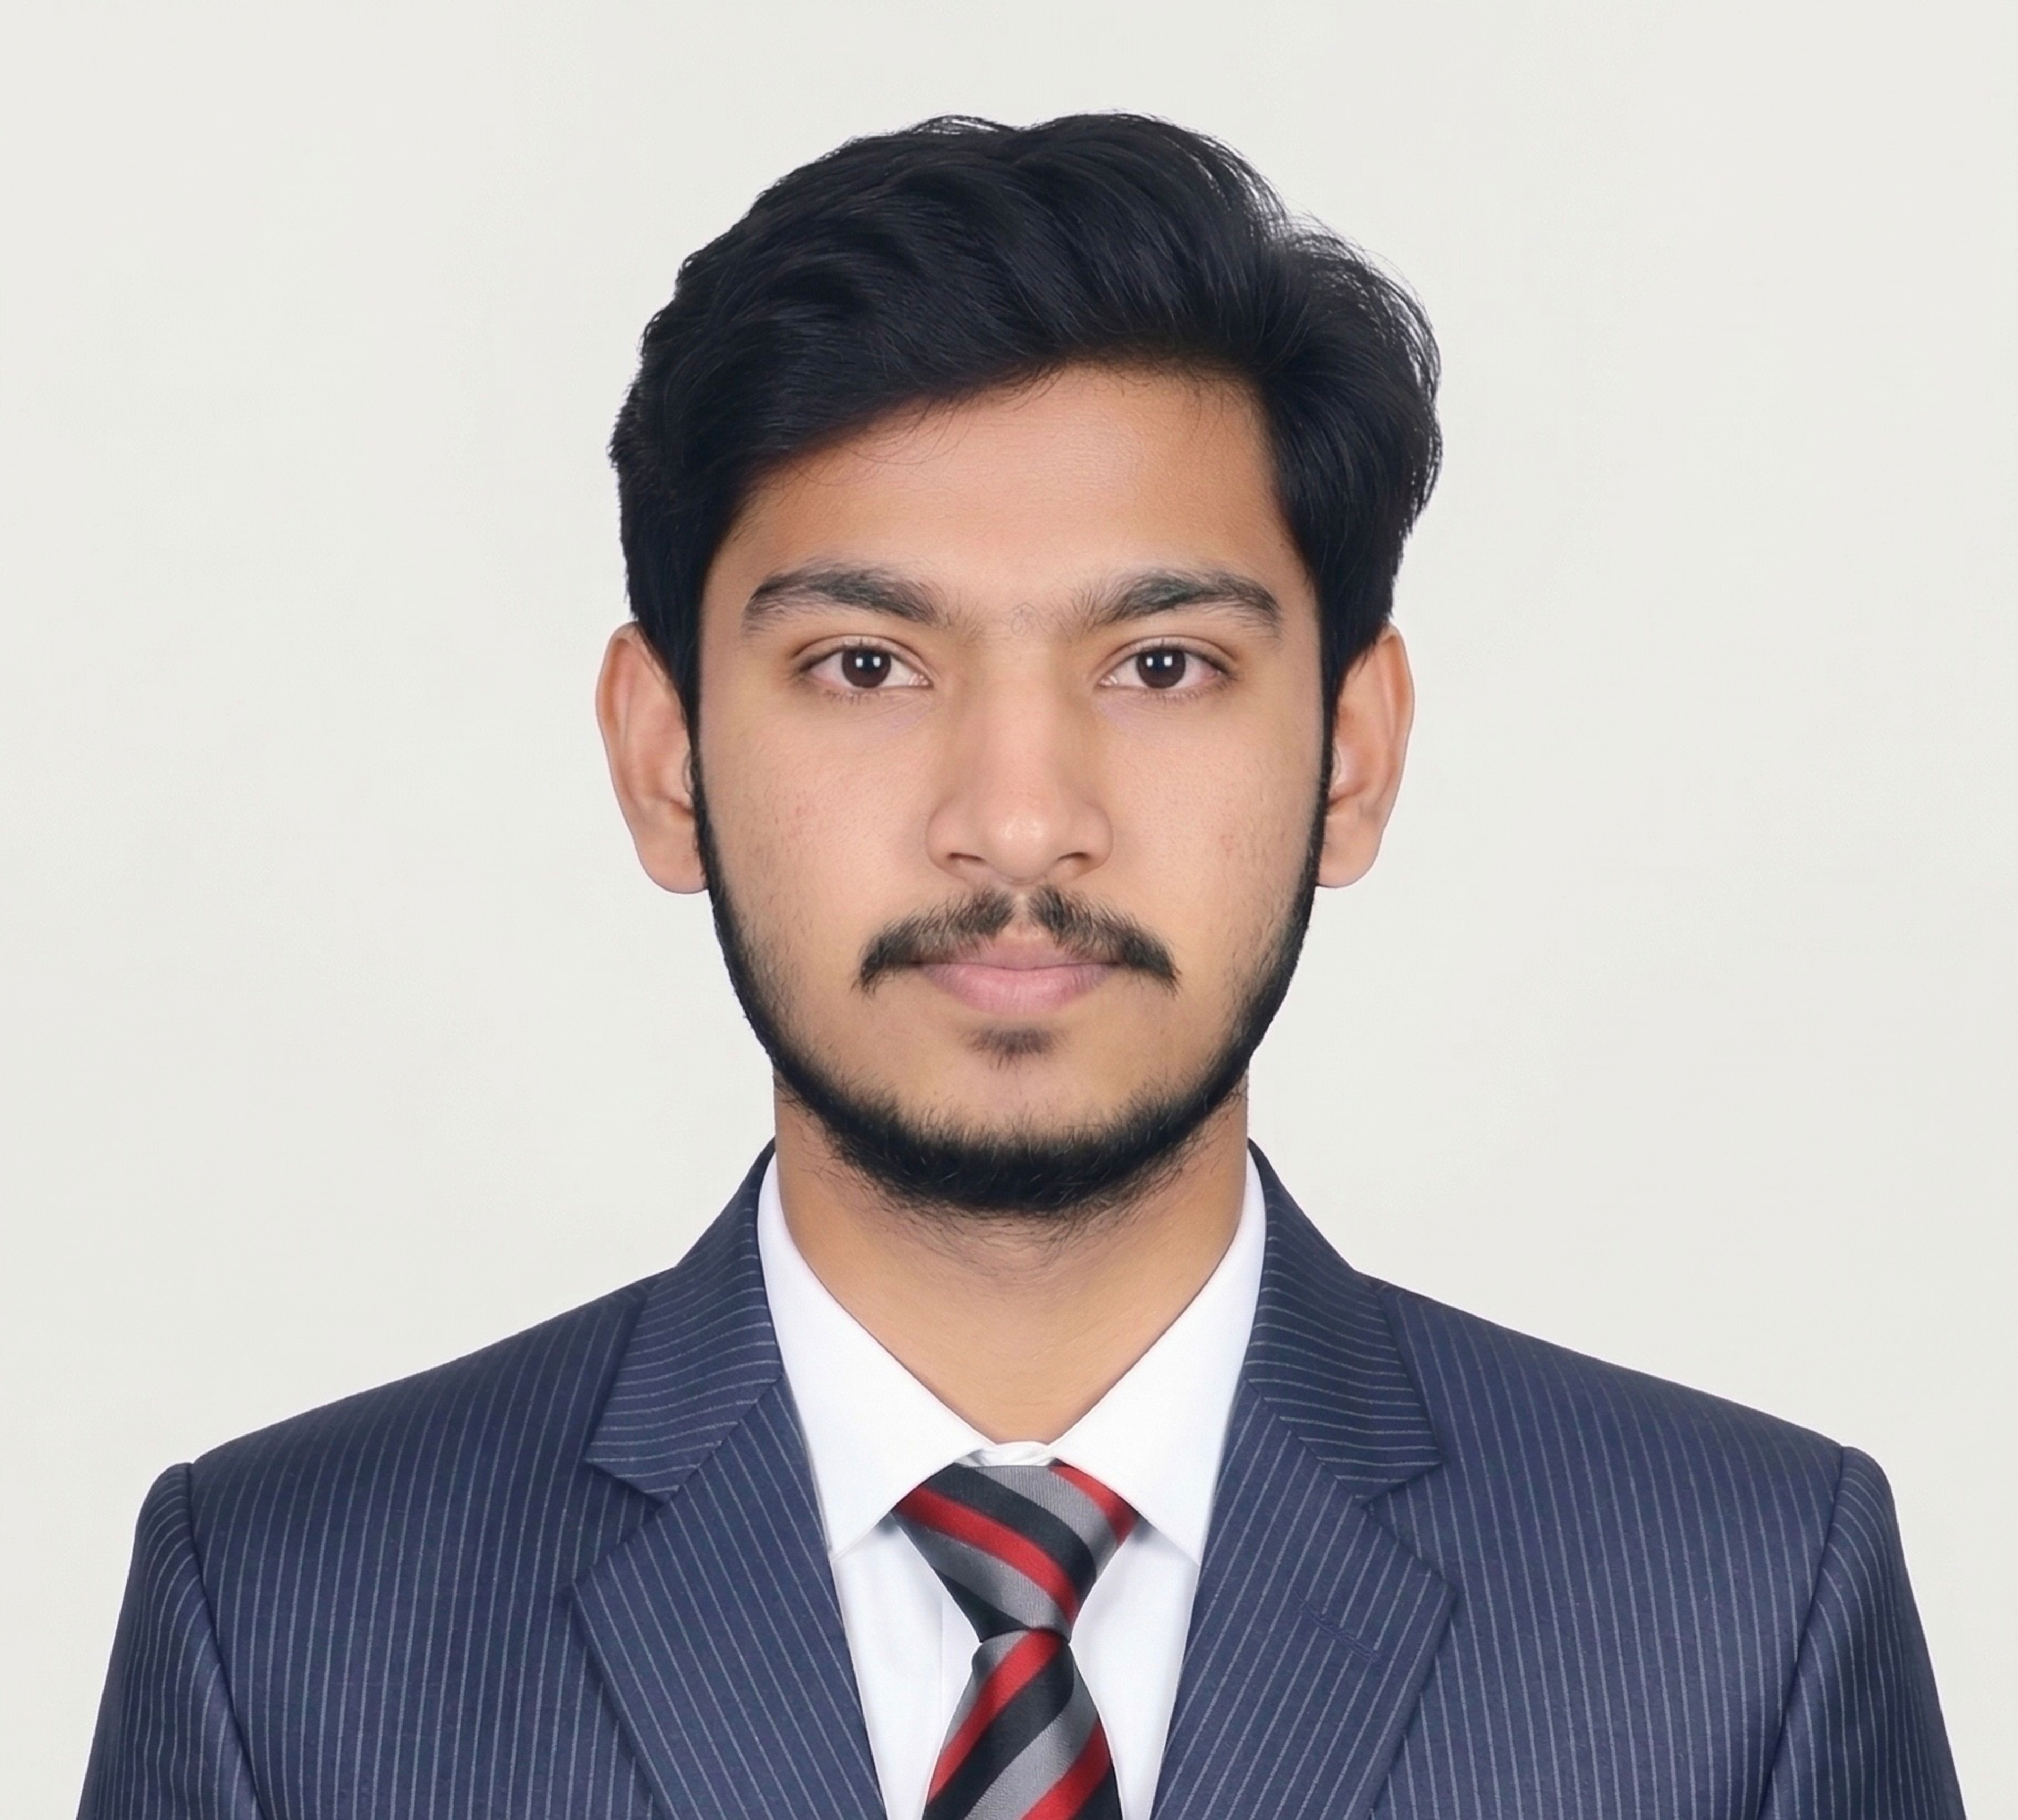
\includegraphics[width=1in,height=1.25in,clip,keepaspectratio]{Author1.pdf}}]{Gonugondla Veera Manikanta}
is pursuing the B.Tech. degree in electrical and electronics engineering at the Manipal Institute of Technology, Manipal Academy of Higher Education, Manipal, India, and is concurrently pursuing the B.S. degree in electronic systems at the Indian Institute of Technology (IIT) Madras through its online B.S. programme. His research interests lie at the intersection of artificial intelligence, machine learning, and embedded systems, with a particular focus on privacy-preserving edge-AI platforms, neural-processing-unit deployment of vision models, and real-time single-board-computer systems. He has worked on FPGA-based digital design, RISC-V processor implementations, Raspberry Pi and ESP32-class embedded builds, and the integration of deep-learning inference with hardware-accelerated pipelines. His broader interests include practical, self-hosted alternatives to cloud-dependent consumer electronics, with an emphasis on measurable system-level behaviour under concurrent load.
\end{IEEEbiography}

\vspace*{-25\baselineskip}
\begin{IEEEbiography}[{
\includegraphics[width=1in,height=1.25in,clip,keepaspectratio]{Author2.pdf}}]{Swathi Tangi}
obtained her B.Tech. in electrical and electronics engineering, followed by her M.Tech. and Ph.D. from the National Institute of Technology Karn
ataka, Surathkal, India. She is currently serving as a faculty member in the School of Electrical Engineering at Manipal Institute of Technology
, Manipal Academy of Higher Education, Manipal. She has guided several student projects and has also mentored multiple global internship project
s under IAESTE and AIESEC. Additionally, she serves as a Doctoral Advisory Committee member for Ph.D. research scholars. Her research interests
include smart grids, distributed generation, electric vehicles, power systems, power system protection, embedded systems, and cybersecurity.
\end{IEEEbiography}

\EOD

\end{document}
